% Options for packages loaded elsewhere
\PassOptionsToPackage{unicode}{hyperref}
\PassOptionsToPackage{hyphens}{url}
%
\documentclass[
]{article}
\usepackage{lmodern}
\usepackage{amssymb,amsmath}
\usepackage{ifxetex,ifluatex}
\ifnum 0\ifxetex 1\fi\ifluatex 1\fi=0 % if pdftex
  \usepackage[T1]{fontenc}
  \usepackage[utf8]{inputenc}
  \usepackage{textcomp} % provide euro and other symbols
\else % if luatex or xetex
  \usepackage{unicode-math}
  \defaultfontfeatures{Scale=MatchLowercase}
  \defaultfontfeatures[\rmfamily]{Ligatures=TeX,Scale=1}
\fi
% Use upquote if available, for straight quotes in verbatim environments
\IfFileExists{upquote.sty}{\usepackage{upquote}}{}
\IfFileExists{microtype.sty}{% use microtype if available
  \usepackage[]{microtype}
  \UseMicrotypeSet[protrusion]{basicmath} % disable protrusion for tt fonts
}{}
\makeatletter
\@ifundefined{KOMAClassName}{% if non-KOMA class
  \IfFileExists{parskip.sty}{%
    \usepackage{parskip}
  }{% else
    \setlength{\parindent}{0pt}
    \setlength{\parskip}{6pt plus 2pt minus 1pt}}
}{% if KOMA class
  \KOMAoptions{parskip=half}}
\makeatother
\usepackage{xcolor}
\IfFileExists{xurl.sty}{\usepackage{xurl}}{} % add URL line breaks if available
\IfFileExists{bookmark.sty}{\usepackage{bookmark}}{\usepackage{hyperref}}
\hypersetup{
  pdftitle={Covid Data Project},
  pdfauthor={Ekimetrics},
  hidelinks,
  pdfcreator={LaTeX via pandoc}}
\urlstyle{same} % disable monospaced font for URLs
\usepackage[margin=1in]{geometry}
\usepackage{color}
\usepackage{fancyvrb}
\newcommand{\VerbBar}{|}
\newcommand{\VERB}{\Verb[commandchars=\\\{\}]}
\DefineVerbatimEnvironment{Highlighting}{Verbatim}{commandchars=\\\{\}}
% Add ',fontsize=\small' for more characters per line
\usepackage{framed}
\definecolor{shadecolor}{RGB}{248,248,248}
\newenvironment{Shaded}{\begin{snugshade}}{\end{snugshade}}
\newcommand{\AlertTok}[1]{\textcolor[rgb]{0.94,0.16,0.16}{#1}}
\newcommand{\AnnotationTok}[1]{\textcolor[rgb]{0.56,0.35,0.01}{\textbf{\textit{#1}}}}
\newcommand{\AttributeTok}[1]{\textcolor[rgb]{0.77,0.63,0.00}{#1}}
\newcommand{\BaseNTok}[1]{\textcolor[rgb]{0.00,0.00,0.81}{#1}}
\newcommand{\BuiltInTok}[1]{#1}
\newcommand{\CharTok}[1]{\textcolor[rgb]{0.31,0.60,0.02}{#1}}
\newcommand{\CommentTok}[1]{\textcolor[rgb]{0.56,0.35,0.01}{\textit{#1}}}
\newcommand{\CommentVarTok}[1]{\textcolor[rgb]{0.56,0.35,0.01}{\textbf{\textit{#1}}}}
\newcommand{\ConstantTok}[1]{\textcolor[rgb]{0.00,0.00,0.00}{#1}}
\newcommand{\ControlFlowTok}[1]{\textcolor[rgb]{0.13,0.29,0.53}{\textbf{#1}}}
\newcommand{\DataTypeTok}[1]{\textcolor[rgb]{0.13,0.29,0.53}{#1}}
\newcommand{\DecValTok}[1]{\textcolor[rgb]{0.00,0.00,0.81}{#1}}
\newcommand{\DocumentationTok}[1]{\textcolor[rgb]{0.56,0.35,0.01}{\textbf{\textit{#1}}}}
\newcommand{\ErrorTok}[1]{\textcolor[rgb]{0.64,0.00,0.00}{\textbf{#1}}}
\newcommand{\ExtensionTok}[1]{#1}
\newcommand{\FloatTok}[1]{\textcolor[rgb]{0.00,0.00,0.81}{#1}}
\newcommand{\FunctionTok}[1]{\textcolor[rgb]{0.00,0.00,0.00}{#1}}
\newcommand{\ImportTok}[1]{#1}
\newcommand{\InformationTok}[1]{\textcolor[rgb]{0.56,0.35,0.01}{\textbf{\textit{#1}}}}
\newcommand{\KeywordTok}[1]{\textcolor[rgb]{0.13,0.29,0.53}{\textbf{#1}}}
\newcommand{\NormalTok}[1]{#1}
\newcommand{\OperatorTok}[1]{\textcolor[rgb]{0.81,0.36,0.00}{\textbf{#1}}}
\newcommand{\OtherTok}[1]{\textcolor[rgb]{0.56,0.35,0.01}{#1}}
\newcommand{\PreprocessorTok}[1]{\textcolor[rgb]{0.56,0.35,0.01}{\textit{#1}}}
\newcommand{\RegionMarkerTok}[1]{#1}
\newcommand{\SpecialCharTok}[1]{\textcolor[rgb]{0.00,0.00,0.00}{#1}}
\newcommand{\SpecialStringTok}[1]{\textcolor[rgb]{0.31,0.60,0.02}{#1}}
\newcommand{\StringTok}[1]{\textcolor[rgb]{0.31,0.60,0.02}{#1}}
\newcommand{\VariableTok}[1]{\textcolor[rgb]{0.00,0.00,0.00}{#1}}
\newcommand{\VerbatimStringTok}[1]{\textcolor[rgb]{0.31,0.60,0.02}{#1}}
\newcommand{\WarningTok}[1]{\textcolor[rgb]{0.56,0.35,0.01}{\textbf{\textit{#1}}}}
\usepackage{graphicx,grffile}
\makeatletter
\def\maxwidth{\ifdim\Gin@nat@width>\linewidth\linewidth\else\Gin@nat@width\fi}
\def\maxheight{\ifdim\Gin@nat@height>\textheight\textheight\else\Gin@nat@height\fi}
\makeatother
% Scale images if necessary, so that they will not overflow the page
% margins by default, and it is still possible to overwrite the defaults
% using explicit options in \includegraphics[width, height, ...]{}
\setkeys{Gin}{width=\maxwidth,height=\maxheight,keepaspectratio}
% Set default figure placement to htbp
\makeatletter
\def\fps@figure{htbp}
\makeatother
\setlength{\emergencystretch}{3em} % prevent overfull lines
\providecommand{\tightlist}{%
  \setlength{\itemsep}{0pt}\setlength{\parskip}{0pt}}
\setcounter{secnumdepth}{-\maxdimen} % remove section numbering
\usepackage{amsmath}
\usepackage{booktabs}
\usepackage{caption}
\usepackage{longtable}

\title{Covid Data Project}
\author{Ekimetrics}
\date{4/29/2020}

\begin{document}
\maketitle

Aaron of Py-Tips fame and I have decided to offer up a little project.
We're going to be taking a look at some COVID-19 data provided by Johns
Hopkins and put together by Github which can be found here:
\url{https:/github.com/datasets/covid-19}.

Ohhh github\ldots well might as throw in a little git lesson here also.

Everyone spin up their cmd -

\begin{verbatim}
1. Navigate to where you'd like to store these files
    For me that's `cd "OneDrive - Ekimetrics\Documents\Non-Project Work"`
2. Make a new folder for the R file and data
    mkdir CovidProject
3. Navigate into that file
\end{verbatim}

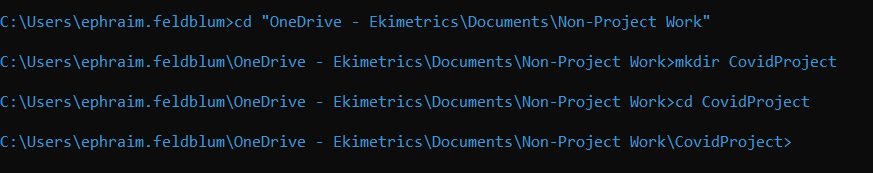
\includegraphics{1.png}

\begin{verbatim}
4. Open the github link and press the Green "Clone or Download" Button
5. In CMD type `git clone [insert link here from last step]
6. take a look at whats been downloaded
    Can just use `tree` here
7. Okay so what we probably want to do is move the data out to the main folder and then delete "covid-19" folder
    `move covid-19\data` # moves the data
    `RMDIR /Q/S covid-19` # Q = quiet mode, won't ask any questions, S = all files and folders within that
8. While you're at it:  
    Make a new folder for your outputs: `mkdir outputs`
\end{verbatim}

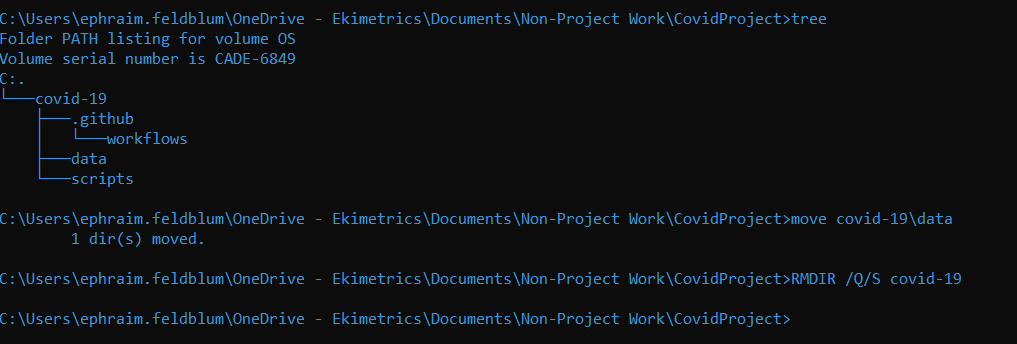
\includegraphics{2.png}

So all together thats: ps feel free to keep the other items, it allows
you to look back in time of this data.

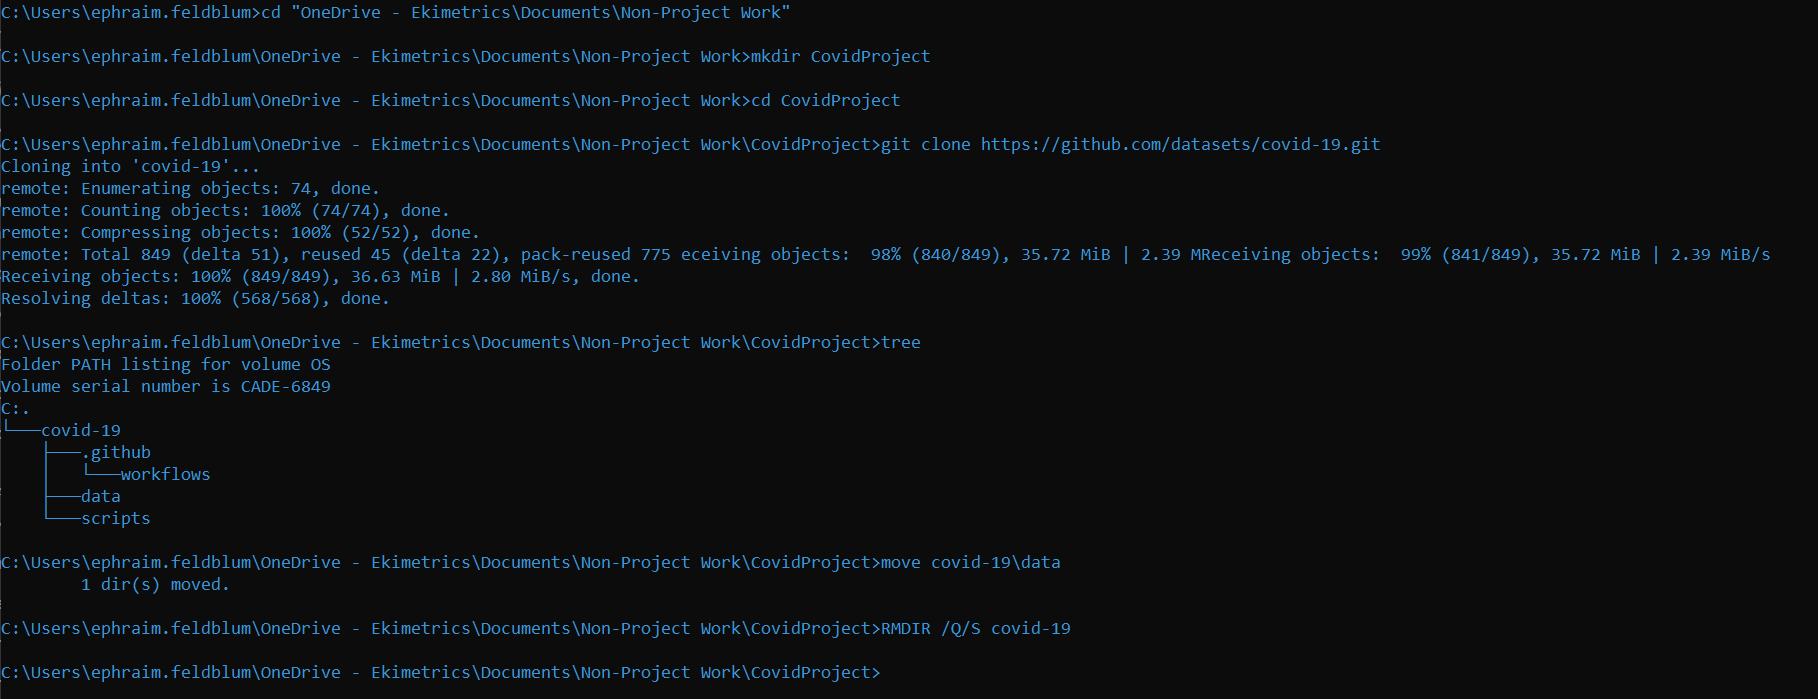
\includegraphics{3.png}

\begin{Shaded}
\begin{Highlighting}[]
\KeywordTok{library}\NormalTok{(tidyverse)}
\KeywordTok{library}\NormalTok{(purrr)}
\KeywordTok{library}\NormalTok{(stringr)}
\KeywordTok{library}\NormalTok{(magrittr)}
\KeywordTok{library}\NormalTok{(janitor)}

\KeywordTok{library}\NormalTok{(zoo)}
\KeywordTok{library}\NormalTok{(modelr)}

\KeywordTok{library}\NormalTok{(gghighlight)}
\KeywordTok{library}\NormalTok{(scales)}

\KeywordTok{library}\NormalTok{(patchwork) }\CommentTok{# arrange plots}
\KeywordTok{library}\NormalTok{(gt) }\CommentTok{# make some nicer looking tables}


\CommentTok{# Ref: https://5harad.com/mse125/r/visualization_code.html}
\NormalTok{addUnits <-}\StringTok{ }\ControlFlowTok{function}\NormalTok{(n) \{}
\NormalTok{  labels <-}\StringTok{ }\KeywordTok{ifelse}\NormalTok{(n }\OperatorTok{<}\StringTok{ }\DecValTok{1000}\NormalTok{, n,  }\CommentTok{# less than thousands}
                   \KeywordTok{ifelse}\NormalTok{(n }\OperatorTok{<}\StringTok{ }\FloatTok{1e6}\NormalTok{, }\KeywordTok{paste0}\NormalTok{(}\KeywordTok{round}\NormalTok{(n}\OperatorTok{/}\FloatTok{1e3}\NormalTok{), }\StringTok{'k'}\NormalTok{),  }\CommentTok{# in thousands}
                          \KeywordTok{ifelse}\NormalTok{(n }\OperatorTok{<}\StringTok{ }\FloatTok{1e9}\NormalTok{, }\KeywordTok{paste0}\NormalTok{(}\KeywordTok{round}\NormalTok{(n}\OperatorTok{/}\FloatTok{1e6}\NormalTok{), }\StringTok{'M'}\NormalTok{),  }\CommentTok{# in millions}
                                 \KeywordTok{ifelse}\NormalTok{(n }\OperatorTok{<}\StringTok{ }\FloatTok{1e12}\NormalTok{, }\KeywordTok{paste0}\NormalTok{(}\KeywordTok{round}\NormalTok{(n}\OperatorTok{/}\FloatTok{1e9}\NormalTok{), }\StringTok{'B'}\NormalTok{), }\CommentTok{# in billions}
                                        \StringTok{'too big!'}
\NormalTok{                                 ))))}
  \KeywordTok{return}\NormalTok{(labels)}
\NormalTok{\}}

 \KeywordTok{scale_y_continuous}\NormalTok{(}\DataTypeTok{labels =}\NormalTok{ addUnits) }
\end{Highlighting}
\end{Shaded}

\begin{verbatim}
## <ScaleContinuousPosition>
##  Range:  
##  Limits:    0 --    1
\end{verbatim}

\begin{Shaded}
\begin{Highlighting}[]
\NormalTok{Eki_theme <-}\StringTok{ }\KeywordTok{theme}\NormalTok{(}\DataTypeTok{panel.grid.minor =} \KeywordTok{element_blank}\NormalTok{(),}
                   \DataTypeTok{panel.grid.major =} \KeywordTok{element_blank}\NormalTok{(),}
                   \DataTypeTok{axis.ticks =} \KeywordTok{element_blank}\NormalTok{(),}
                   \DataTypeTok{panel.background =} \KeywordTok{element_rect}\NormalTok{(}\DataTypeTok{fill =} \StringTok{"transparent"}\NormalTok{,}\DataTypeTok{colour =} \OtherTok{NA}\NormalTok{),}
                   \DataTypeTok{plot.background =} \KeywordTok{element_rect}\NormalTok{(}\DataTypeTok{fill =} \StringTok{"transparent"}\NormalTok{,}\DataTypeTok{colour =} \OtherTok{NA}\NormalTok{))}
\end{Highlighting}
\end{Shaded}

\hypertarget{whats-the-point-of-this-exercise}{%
\section{What's the point of this
exercise?}\label{whats-the-point-of-this-exercise}}

I took as a chance to show off both what we have looked at so far and
show off a few items coming in the next few weeks to show you how these
small bits and bobs can be combined into something.

\hypertarget{formatting}{%
\subsubsection{Formatting:}\label{formatting}}

I'm working on this document thinking it's somewhere between exploration
and being ready to show to somebody - aka I'll put some time into making
it look nice but not too much.

\hypertarget{step-1-what-do-i-have}{%
\section{Step 1: What do I have?}\label{step-1-what-do-i-have}}

Okay, I've been given a folder of random data files. My plan is to try
and take a peak at some of them but there first thing I need to decided
is, ``what is useful to me here?''

Sometimes you might know what you want to do already, but, currently,
I'm flying blind - part of the beauty of R-tips.

\begin{Shaded}
\begin{Highlighting}[]
\CommentTok{# checking my working directory is where I want it to be.}
\KeywordTok{getwd}\NormalTok{()}
\end{Highlighting}
\end{Shaded}

\begin{verbatim}
## [1] "/home/effi/Documents/git to add items/CovidProject/Other shit"
\end{verbatim}

\begin{Shaded}
\begin{Highlighting}[]
\KeywordTok{list.files}\NormalTok{(}\StringTok{"data"}\NormalTok{)}
\end{Highlighting}
\end{Shaded}

\begin{verbatim}
## [1] "countries-aggregated.csv"          "key-countries-pivoted.csv"        
## [3] "reference.csv"                     "time-series-19-covid-combined.csv"
## [5] "us_confirmed.csv"                  "us_deaths.csv"                    
## [7] "worldwide-aggregated.csv"
\end{verbatim}

So, I'm not positive yet but I'm thinking I'll focus in on the US.

\begin{Shaded}
\begin{Highlighting}[]
\CommentTok{# so I split out all the US files}
\NormalTok{fileNames <-}\StringTok{ }\KeywordTok{list.files}\NormalTok{(}\StringTok{"data"}\NormalTok{)}
\NormalTok{usFilesLoc <-}\StringTok{ }\KeywordTok{grep}\NormalTok{(}\StringTok{"us"}\NormalTok{,fileNames) }\CommentTok{# selecting the indexes of the us files}
\NormalTok{usFiles <-}\StringTok{ }\NormalTok{fileNames[usFilesLoc]}
\NormalTok{otherFiles <-}\StringTok{ }\NormalTok{fileNames[}\OperatorTok{-}\NormalTok{usFilesLoc]}
\end{Highlighting}
\end{Shaded}

All the files are csvs which is nice.

\begin{Shaded}
\begin{Highlighting}[]
\CommentTok{# Im gonna check out the "other files" first}
\KeywordTok{head}\NormalTok{(}\KeywordTok{read_csv}\NormalTok{(}\KeywordTok{paste0}\NormalTok{(}\StringTok{"data/"}\NormalTok{,otherFiles[}\DecValTok{4}\NormalTok{])),}\DecValTok{25}\NormalTok{)}
\end{Highlighting}
\end{Shaded}

\begin{verbatim}
## Parsed with column specification:
## cols(
##   Date = col_date(format = ""),
##   `Country/Region` = col_character(),
##   `Province/State` = col_character(),
##   Lat = col_double(),
##   Long = col_double(),
##   Confirmed = col_double(),
##   Recovered = col_double(),
##   Deaths = col_double()
## )
\end{verbatim}

\begin{verbatim}
## # A tibble: 25 x 8
##    Date       `Country/Region` `Province/State`   Lat  Long Confirmed Recovered
##    <date>     <chr>            <chr>            <dbl> <dbl>     <dbl>     <dbl>
##  1 2020-01-22 Afghanistan      <NA>                33    65         0         0
##  2 2020-01-23 Afghanistan      <NA>                33    65         0         0
##  3 2020-01-24 Afghanistan      <NA>                33    65         0         0
##  4 2020-01-25 Afghanistan      <NA>                33    65         0         0
##  5 2020-01-26 Afghanistan      <NA>                33    65         0         0
##  6 2020-01-27 Afghanistan      <NA>                33    65         0         0
##  7 2020-01-28 Afghanistan      <NA>                33    65         0         0
##  8 2020-01-29 Afghanistan      <NA>                33    65         0         0
##  9 2020-01-30 Afghanistan      <NA>                33    65         0         0
## 10 2020-01-31 Afghanistan      <NA>                33    65         0         0
## # ... with 15 more rows, and 1 more variable: Deaths <dbl>
\end{verbatim}

\begin{Shaded}
\begin{Highlighting}[]
\NormalTok{otherFilesGuide <-}\StringTok{ }\KeywordTok{tribble}\NormalTok{( }\OperatorTok{~}\NormalTok{file, }\OperatorTok{~}\NormalTok{contains,}
\NormalTok{         otherFiles[}\DecValTok{1}\NormalTok{],}\StringTok{"Overall Countries with Confirmed, Recovered, and Deaths"}\NormalTok{,}
\NormalTok{         otherFiles[}\DecValTok{2}\NormalTok{], }\StringTok{"pivoted deaths for US, UK, Italy, France, Germ, Spa, Iran"}\NormalTok{,}
\NormalTok{         otherFiles[}\DecValTok{3}\NormalTok{], }\StringTok{"Countries with codes, lat&lon, population"}\NormalTok{,}
\NormalTok{         otherFiles[}\DecValTok{4}\NormalTok{], }\StringTok{"Countries with confirmed, recovered, deaths - same as 1 with province/state"}\NormalTok{,}
\NormalTok{         otherFiles[}\DecValTok{5}\NormalTok{], }\StringTok{"worldwide total confirmed, recovered, deaths, increase rate"}
\NormalTok{         )}
\end{Highlighting}
\end{Shaded}

I did the above manually in R and took a few moments to check out each
DF.

\hypertarget{us-data}{%
\subsection{US Data:}\label{us-data}}

\begin{Shaded}
\begin{Highlighting}[]
\CommentTok{# Because I think I'm going to focus on the US let's load all those files in}

\NormalTok{us_confirmed <-}\StringTok{ }\KeywordTok{read_csv}\NormalTok{(}\KeywordTok{paste0}\NormalTok{(}\StringTok{"data/"}\NormalTok{, usFiles[}\DecValTok{1}\NormalTok{]))}
\end{Highlighting}
\end{Shaded}

\begin{verbatim}
## Parsed with column specification:
## cols(
##   UID = col_double(),
##   iso2 = col_character(),
##   iso3 = col_character(),
##   code3 = col_double(),
##   FIPS = col_double(),
##   Admin2 = col_character(),
##   Lat = col_double(),
##   Combined_Key = col_character(),
##   Date = col_date(format = ""),
##   Case = col_double(),
##   Long = col_double(),
##   `Country/Region` = col_character(),
##   `Province/State` = col_character()
## )
\end{verbatim}

\begin{Shaded}
\begin{Highlighting}[]
\NormalTok{us_deaths <-}\StringTok{ }\KeywordTok{read_csv}\NormalTok{(}\KeywordTok{paste0}\NormalTok{(}\StringTok{"data/"}\NormalTok{, usFiles[}\DecValTok{2}\NormalTok{]))}
\end{Highlighting}
\end{Shaded}

\begin{verbatim}
## Parsed with column specification:
## cols(
##   UID = col_double(),
##   iso2 = col_character(),
##   iso3 = col_character(),
##   code3 = col_double(),
##   FIPS = col_double(),
##   Admin2 = col_character(),
##   Lat = col_double(),
##   Combined_Key = col_character(),
##   Population = col_double(),
##   Date = col_date(format = ""),
##   Case = col_double(),
##   Long = col_double(),
##   `Country/Region` = col_character(),
##   `Province/State` = col_character()
## )
\end{verbatim}

\begin{Shaded}
\begin{Highlighting}[]
\NormalTok{us_confirmed }\OperatorTok
\StringTok{  }\KeywordTok{head}\NormalTok{() }\OperatorTok
\StringTok{  }\NormalTok{gt }\OperatorTok\StringTok{ }
\StringTok{  }\KeywordTok{tab_header}\NormalTok{(}
    \DataTypeTok{title =} \KeywordTok{md}\NormalTok{(}\StringTok{"Confirmed US Cases"}\NormalTok{),}\DataTypeTok{subtitle =} \KeywordTok{md}\NormalTok{(}\StringTok{"&nbsp;"}\NormalTok{))}
\end{Highlighting}
\end{Shaded}

\captionsetup[table]{labelformat=empty,skip=1pt}
\begin{longtable}{rllrrlrllrrll}
\caption*{
\large Confirmed US Cases\\ 
\small ~\\ 
} \\ 
\toprule
UID & iso2 & iso3 & code3 & FIPS & Admin2 & Lat & Combined\_Key & Date & Case & Long & Country/Region & Province/State \\ 
\midrule
16 & AS & ASM & 16 & 60 & NA & -14.271 & American Samoa, US & 2020-01-22 & 0 & -170.132 & US & American Samoa \\ 
16 & AS & ASM & 16 & 60 & NA & -14.271 & American Samoa, US & 2020-01-23 & 0 & -170.132 & US & American Samoa \\ 
16 & AS & ASM & 16 & 60 & NA & -14.271 & American Samoa, US & 2020-01-24 & 0 & -170.132 & US & American Samoa \\ 
16 & AS & ASM & 16 & 60 & NA & -14.271 & American Samoa, US & 2020-01-25 & 0 & -170.132 & US & American Samoa \\ 
16 & AS & ASM & 16 & 60 & NA & -14.271 & American Samoa, US & 2020-01-26 & 0 & -170.132 & US & American Samoa \\ 
16 & AS & ASM & 16 & 60 & NA & -14.271 & American Samoa, US & 2020-01-27 & 0 & -170.132 & US & American Samoa \\ 
\bottomrule
\end{longtable}

\begin{Shaded}
\begin{Highlighting}[]
\NormalTok{us_deaths }\OperatorTok
\StringTok{  }\KeywordTok{head}\NormalTok{()}\OperatorTok
\StringTok{  }\NormalTok{gt }\OperatorTok
\StringTok{  }\KeywordTok{tab_header}\NormalTok{(}
    \DataTypeTok{title =} \KeywordTok{md}\NormalTok{(}\StringTok{"Confirmed US Deaths"}\NormalTok{),}\DataTypeTok{subtitle =} \KeywordTok{md}\NormalTok{(}\StringTok{"&nbsp;"}\NormalTok{))}
\end{Highlighting}
\end{Shaded}

\captionsetup[table]{labelformat=empty,skip=1pt}
\begin{longtable}{rllrrlrlrlrrll}
\caption*{
\large Confirmed US Deaths\\ 
\small ~\\ 
} \\ 
\toprule
UID & iso2 & iso3 & code3 & FIPS & Admin2 & Lat & Combined\_Key & Population & Date & Case & Long & Country/Region & Province/State \\ 
\midrule
16 & AS & ASM & 16 & 60 & NA & -14.271 & American Samoa, US & 55641 & 2020-01-22 & 0 & -170.132 & US & American Samoa \\ 
16 & AS & ASM & 16 & 60 & NA & -14.271 & American Samoa, US & 55641 & 2020-01-23 & 0 & -170.132 & US & American Samoa \\ 
16 & AS & ASM & 16 & 60 & NA & -14.271 & American Samoa, US & 55641 & 2020-01-24 & 0 & -170.132 & US & American Samoa \\ 
16 & AS & ASM & 16 & 60 & NA & -14.271 & American Samoa, US & 55641 & 2020-01-25 & 0 & -170.132 & US & American Samoa \\ 
16 & AS & ASM & 16 & 60 & NA & -14.271 & American Samoa, US & 55641 & 2020-01-26 & 0 & -170.132 & US & American Samoa \\ 
16 & AS & ASM & 16 & 60 & NA & -14.271 & American Samoa, US & 55641 & 2020-01-27 & 0 & -170.132 & US & American Samoa \\ 
\bottomrule
\end{longtable}

So one of my first questions here is whether I can just merger these two
dfs together? They seem pretty identical. Some quick checks:

\begin{Shaded}
\begin{Highlighting}[]
\KeywordTok{ncol}\NormalTok{(us_confirmed) }\OperatorTok{==}\StringTok{ }\KeywordTok{ncol}\NormalTok{(us_deaths) }\CommentTok{# oo so they already don't have the same number of columns}
\end{Highlighting}
\end{Shaded}

\begin{verbatim}
## [1] FALSE
\end{verbatim}

\begin{Shaded}
\begin{Highlighting}[]
\KeywordTok{ncol}\NormalTok{(us_confirmed) }\OperatorTok{>}\StringTok{ }\KeywordTok{ncol}\NormalTok{(us_deaths) }\CommentTok{# us_deaths have more}
\end{Highlighting}
\end{Shaded}

\begin{verbatim}
## [1] FALSE
\end{verbatim}

\begin{Shaded}
\begin{Highlighting}[]
\KeywordTok{setdiff}\NormalTok{(}\KeywordTok{colnames}\NormalTok{(us_deaths),}\KeywordTok{colnames}\NormalTok{(us_confirmed)) }\CommentTok{#so no population in confirmed}
\end{Highlighting}
\end{Shaded}

\begin{verbatim}
## [1] "Population"
\end{verbatim}

\begin{Shaded}
\begin{Highlighting}[]
\KeywordTok{setdiff}\NormalTok{(}\KeywordTok{colnames}\NormalTok{(us_confirmed),}\KeywordTok{colnames}\NormalTok{(us_deaths)) }\CommentTok{# no differences}
\end{Highlighting}
\end{Shaded}

\begin{verbatim}
## character(0)
\end{verbatim}

\begin{Shaded}
\begin{Highlighting}[]
\KeywordTok{colnames}\NormalTok{(us_deaths)}
\end{Highlighting}
\end{Shaded}

\begin{verbatim}
##  [1] "UID"            "iso2"           "iso3"           "code3"         
##  [5] "FIPS"           "Admin2"         "Lat"            "Combined_Key"  
##  [9] "Population"     "Date"           "Case"           "Long"          
## [13] "Country/Region" "Province/State"
\end{verbatim}

\begin{Shaded}
\begin{Highlighting}[]
\KeywordTok{nrow}\NormalTok{(us_confirmed) }\OperatorTok{==}\StringTok{ }\KeywordTok{nrow}\NormalTok{(us_deaths) }\CommentTok{# same number of rows - makes sense, certain # days for certain # of places}
\end{Highlighting}
\end{Shaded}

\begin{verbatim}
## [1] TRUE
\end{verbatim}

Okay, I think we're pretty ready to just go ahead and rename the values
column. And merge the two files.

\begin{Shaded}
\begin{Highlighting}[]
\NormalTok{us_confirmed <-}\StringTok{ }\NormalTok{dplyr}\OperatorTok{::}\KeywordTok{rename}\NormalTok{(us_confirmed, }\DataTypeTok{confirmed =}\NormalTok{ Case)}
\NormalTok{us_deaths <-}\StringTok{ }\NormalTok{dplyr}\OperatorTok{::}\KeywordTok{rename}\NormalTok{(us_deaths, }\DataTypeTok{deaths =}\NormalTok{ Case)}

\NormalTok{us_data <-}\StringTok{ }\NormalTok{us_confirmed }\OperatorTok
\StringTok{    }\KeywordTok{full_join}\NormalTok{(us_deaths)}\OperatorTok
\StringTok{    }\KeywordTok{pivot_longer}\NormalTok{(}\KeywordTok{c}\NormalTok{(deaths, confirmed), }\DataTypeTok{names_to =} \StringTok{"confirm/deaths"}\NormalTok{, }\DataTypeTok{values_to =} \StringTok{"cumValues"}\NormalTok{)}\OperatorTok
\StringTok{    }\KeywordTok{clean_names}\NormalTok{()}
\end{Highlighting}
\end{Shaded}

\begin{verbatim}
## Joining, by = c("UID", "iso2", "iso3", "code3", "FIPS", "Admin2", "Lat", "Combined_Key", "Date", "Long", "Country/Region", "Province/State")
\end{verbatim}

Let's do some checks on the US data - our primary source:

\begin{Shaded}
\begin{Highlighting}[]
\KeywordTok{library}\NormalTok{(plyr) }\CommentTok{# Im putting this here bc plyr annoys me so Im going to be unloading it at the end of this chunk }
\end{Highlighting}
\end{Shaded}

\begin{verbatim}
## ------------------------------------------------------------------------------
\end{verbatim}

\begin{verbatim}
## You have loaded plyr after dplyr - this is likely to cause problems.
## If you need functions from both plyr and dplyr, please load plyr first, then dplyr:
## library(plyr); library(dplyr)
\end{verbatim}

\begin{verbatim}
## ------------------------------------------------------------------------------
\end{verbatim}

\begin{verbatim}
## 
## Attaching package: 'plyr'
\end{verbatim}

\begin{verbatim}
## The following objects are masked from 'package:dplyr':
## 
##     arrange, count, desc, failwith, id, mutate, rename, summarise,
##     summarize
\end{verbatim}

\begin{verbatim}
## The following object is masked from 'package:purrr':
## 
##     compact
\end{verbatim}

\begin{Shaded}
\begin{Highlighting}[]
\CommentTok{# any missing values?}

\KeywordTok{ldply}\NormalTok{(us_data,}\ControlFlowTok{function}\NormalTok{(x)  }\CommentTok{# this function:}
    \KeywordTok{sum}\NormalTok{(}\KeywordTok{is.na}\NormalTok{(x)) }\OperatorTok{/}\StringTok{ }\KeywordTok{nrow}\NormalTok{(us_data))}\OperatorTok
\StringTok{    }\NormalTok{dplyr}\OperatorTok{::}\KeywordTok{rename}\NormalTok{(}\DataTypeTok{Variable =} \StringTok{`}\DataTypeTok{.id}\StringTok{`}\NormalTok{, }\StringTok{`}\DataTypeTok{Percent Missing}\StringTok{`}\NormalTok{ =}\StringTok{ }\NormalTok{V1)}\OperatorTok
\StringTok{  }\KeywordTok{arrange}\NormalTok{(}\KeywordTok{desc}\NormalTok{(}\StringTok{`}\DataTypeTok{Percent Missing}\StringTok{`}\NormalTok{))}\OperatorTok
\StringTok{  }\KeywordTok{gt}\NormalTok{()}\OperatorTok
\StringTok{  }\KeywordTok{fmt_percent}\NormalTok{(}
    \DataTypeTok{columns =} \KeywordTok{vars}\NormalTok{(}\StringTok{`}\DataTypeTok{Percent Missing}\StringTok{`}\NormalTok{),}
    \DataTypeTok{decimals =}\DecValTok{3}\NormalTok{)}
\end{Highlighting}
\end{Shaded}

\captionsetup[table]{labelformat=empty,skip=1pt}
\begin{longtable}{lr}
\toprule
Variable & Percent Missing \\ 
\midrule
fips & $0.307\%$ \\ 
admin2 & $0.215\%$ \\ 
uid & $0.031\%$ \\ 
lat & $0.031\%$ \\ 
long & $0.031\%$ \\ 
iso2 & $0.000\%$ \\ 
iso3 & $0.000\%$ \\ 
code3 & $0.000\%$ \\ 
combined\_key & $0.000\%$ \\ 
date & $0.000\%$ \\ 
country\_region & $0.000\%$ \\ 
province\_state & $0.000\%$ \\ 
population & $0.000\%$ \\ 
confirm\_deaths & $0.000\%$ \\ 
cum\_values & $0.000\%$ \\ 
\bottomrule
\end{longtable}

\begin{Shaded}
\begin{Highlighting}[]
\KeywordTok{detach}\NormalTok{(package}\OperatorTok{:}\NormalTok{plyr, }\DataTypeTok{unload=}\OtherTok{TRUE}\NormalTok{)}
\end{Highlighting}
\end{Shaded}

so we're missing around 2\% of the more granular location data

Let's take a peak at those admin areas we're missing:

\begin{Shaded}
\begin{Highlighting}[]
\NormalTok{us_data }\OperatorTok
\StringTok{    }\KeywordTok{filter}\NormalTok{(}\KeywordTok{is.na}\NormalTok{(admin2))}\OperatorTok
\StringTok{    }\KeywordTok{distinct}\NormalTok{(province_state)}
\end{Highlighting}
\end{Shaded}

\begin{verbatim}
## # A tibble: 7 x 1
##   province_state          
##   <chr>                   
## 1 American Samoa          
## 2 Guam                    
## 3 Northern Mariana Islands
## 4 Puerto Rico             
## 5 Virgin Islands          
## 6 Diamond Princess        
## 7 Grand Princess
\end{verbatim}

Alright, every place we're missing more granular data makes
sense\ldots well let's see what areas we're covering with this data set.

\begin{Shaded}
\begin{Highlighting}[]
\CommentTok{# How many areas are we counting}
\NormalTok{us_data }\OperatorTok\StringTok{ }\KeywordTok{distinct}\NormalTok{(province_state) }\CommentTok{# so all the states + dc + some other US stuff (sorry Gman) + two cruise ships}
\end{Highlighting}
\end{Shaded}

\begin{verbatim}
## # A tibble: 58 x 1
##    province_state          
##    <chr>                   
##  1 American Samoa          
##  2 Guam                    
##  3 Northern Mariana Islands
##  4 Puerto Rico             
##  5 Virgin Islands          
##  6 Alabama                 
##  7 Alaska                  
##  8 Arizona                 
##  9 Arkansas                
## 10 California              
## # ... with 48 more rows
\end{verbatim}

\begin{Shaded}
\begin{Highlighting}[]
\NormalTok{us_data }\OperatorTok\StringTok{ }\KeywordTok{distinct}\NormalTok{(admin2) }\CommentTok{# okay so we have 1903 localities }
\end{Highlighting}
\end{Shaded}

\begin{verbatim}
## # A tibble: 1,903 x 1
##    admin2  
##    <chr>   
##  1 <NA>    
##  2 Autauga 
##  3 Baldwin 
##  4 Barbour 
##  5 Bibb    
##  6 Blount  
##  7 Bullock 
##  8 Butler  
##  9 Calhoun 
## 10 Chambers
## # ... with 1,893 more rows
\end{verbatim}

Let's take a look at the amount of localities per state

\begin{Shaded}
\begin{Highlighting}[]
\NormalTok{us_data }\OperatorTok
\StringTok{    }\KeywordTok{distinct}\NormalTok{(admin2, }\DataTypeTok{.keep_all =} \OtherTok{TRUE}\NormalTok{)}\OperatorTok
\StringTok{    }\KeywordTok{select}\NormalTok{(admin2, province_state) }\OperatorTok
\StringTok{    }\KeywordTok{table}\NormalTok{(province_state)}\OperatorTok
\StringTok{    }\KeywordTok{as.data.frame.table}\NormalTok{()}\OperatorTok
\StringTok{    }\KeywordTok{arrange}\NormalTok{(}\OperatorTok{-}\NormalTok{Freq) }\OperatorTok
\StringTok{  }\KeywordTok{head}\NormalTok{(}\DecValTok{15}\NormalTok{)}\OperatorTok\StringTok{  }
\StringTok{  }\KeywordTok{gt}\NormalTok{() }\OperatorTok
\StringTok{  }\KeywordTok{tab_header}\NormalTok{(}
    \DataTypeTok{title =} \KeywordTok{md}\NormalTok{(}\StringTok{"Localities Per State for 15 most Divided"}\NormalTok{),}\DataTypeTok{subtitle =} \KeywordTok{md}\NormalTok{(}\StringTok{"&nbsp;"}\NormalTok{))}
\end{Highlighting}
\end{Shaded}

\captionsetup[table]{labelformat=empty,skip=1pt}
\begin{longtable}{cc}
\caption*{
\large Localities Per State for 15 most Divided\\ 
\small ~\\ 
} \\ 
\toprule
province\_state & Freq \\ 
\midrule
Texas & 161 \\ 
Georgia & 109 \\ 
Virginia & 73 \\ 
Alabama & 69 \\ 
Kansas & 68 \\ 
Michigan & 65 \\ 
North Carolina & 65 \\ 
Minnesota & 62 \\ 
Arkansas & 58 \\ 
California & 57 \\ 
Colorado & 56 \\ 
Kentucky & 56 \\ 
Illinois & 55 \\ 
Florida & 50 \\ 
Louisiana & 48 \\ 
\bottomrule
\end{longtable}

Let's figure out what the max day, as the numbers are cumulative it will
be pretty useful to save that date as a variable instead of tons of
ctrl-c, ctrl-v.

\begin{Shaded}
\begin{Highlighting}[]
\NormalTok{maxDate <-}\StringTok{ }\KeywordTok{max}\NormalTok{(us_data}\OperatorTok{$}\NormalTok{date) }
\end{Highlighting}
\end{Shaded}

It's 2020-04-28 and as of writing this it's the evening of April 29th so
this is probably a good idea because by the time you run this code (or I
rerun to send to you), the date will be different\ldots{} and I made
this document reactive so maybe the first part of this sentence won't
even say April 28th\ldots.

Might as well also see the min date:

\begin{Shaded}
\begin{Highlighting}[]
\KeywordTok{min}\NormalTok{(us_data}\OperatorTok{$}\NormalTok{date)}
\end{Highlighting}
\end{Shaded}

\begin{verbatim}
## [1] "2020-01-22"
\end{verbatim}

\hypertarget{some-graphs}{%
\subsection{Some Graphs}\label{some-graphs}}

Alright let's maybe take a look at some graphs to try and start to get a
handle on this data.

\begin{Shaded}
\begin{Highlighting}[]
\NormalTok{us_data }\OperatorTok
\StringTok{  }\KeywordTok{filter}\NormalTok{(confirm_deaths }\OperatorTok{==}\StringTok{ "confirmed"}\NormalTok{)}\OperatorTok
\StringTok{  }\KeywordTok{group_by}\NormalTok{(date, province_state)}\OperatorTok
\StringTok{  }\KeywordTok{summarise}\NormalTok{(}\DataTypeTok{confirmed =} \KeywordTok{sum}\NormalTok{(cum_values)) }\OperatorTok
\KeywordTok{ggplot}\NormalTok{(}\KeywordTok{aes}\NormalTok{(date,confirmed, }\DataTypeTok{group =}\NormalTok{ province_state)) }\OperatorTok{+}
\StringTok{    }\KeywordTok{geom_line}\NormalTok{(}\DataTypeTok{alpha =} \DecValTok{1}\OperatorTok{/}\DecValTok{3}\NormalTok{)}\OperatorTok{+}
\StringTok{    }\KeywordTok{gghighlight}\NormalTok{(}\KeywordTok{max}\NormalTok{(confirmed) }\OperatorTok{>}\StringTok{ }\DecValTok{40000}\NormalTok{,}
            \DataTypeTok{label_params =} \KeywordTok{list}\NormalTok{(}
                \DataTypeTok{fill =} \OtherTok{NA}\NormalTok{,}
                \DataTypeTok{segment.color =} \StringTok{"light blue"}\NormalTok{,}
                \DataTypeTok{label.size =} \OtherTok{NA}
\NormalTok{            )) }\OperatorTok{+}
\StringTok{    }\KeywordTok{scale_y_continuous}\NormalTok{(}\DataTypeTok{labels =}\NormalTok{ addUnits) }\OperatorTok{+}
\StringTok{  }\NormalTok{Eki_theme }\OperatorTok{+}
\StringTok{  }\KeywordTok{ggtitle}\NormalTok{(}\StringTok{"Confirmed Cases Per State"}\NormalTok{)}
\end{Highlighting}
\end{Shaded}

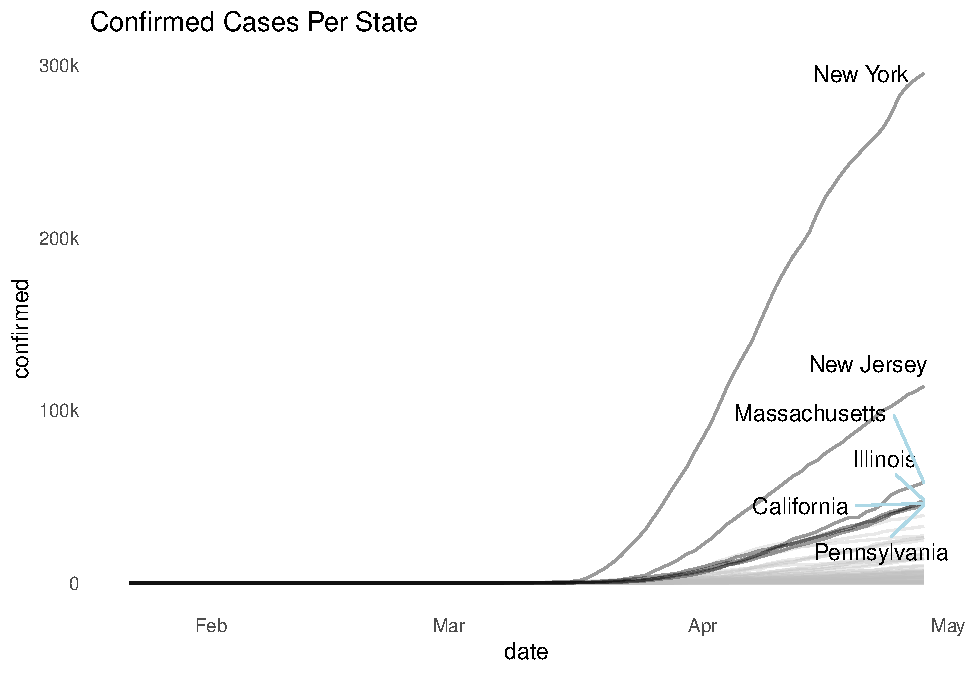
\includegraphics{Project-1---Covid---Final_files/figure-latex/unnamed-chunk-15-1.pdf}

Let's split NYC - as we should cuz it be the home.

\begin{Shaded}
\begin{Highlighting}[]
\NormalTok{us_data }\OperatorTok
\StringTok{  }\KeywordTok{filter}\NormalTok{(confirm_deaths }\OperatorTok{==}\StringTok{ "confirmed"}\NormalTok{)}\OperatorTok
\StringTok{  }\KeywordTok{mutate}\NormalTok{(}\DataTypeTok{province_state =} \KeywordTok{ifelse}\NormalTok{(admin2 }\OperatorTok{==}\StringTok{ "New York"}\NormalTok{, }\StringTok{"NYC"}\NormalTok{, province_state)) }\OperatorTok
\StringTok{  }\KeywordTok{group_by}\NormalTok{(date, province_state)}\OperatorTok
\StringTok{  }\KeywordTok{summarise}\NormalTok{(}\DataTypeTok{confirmed =} \KeywordTok{sum}\NormalTok{(cum_values)) }\OperatorTok
\KeywordTok{ggplot}\NormalTok{(}\KeywordTok{aes}\NormalTok{(date,confirmed, }\DataTypeTok{group =}\NormalTok{ province_state)) }\OperatorTok{+}
\StringTok{    }\KeywordTok{geom_line}\NormalTok{(}\DataTypeTok{alpha =} \DecValTok{1}\OperatorTok{/}\DecValTok{3}\NormalTok{)}\OperatorTok{+}
\StringTok{    }\KeywordTok{gghighlight}\NormalTok{(}\KeywordTok{max}\NormalTok{(confirmed) }\OperatorTok{>}\StringTok{ }\DecValTok{40000}\NormalTok{,}
            \DataTypeTok{label_params =} \KeywordTok{list}\NormalTok{(}
                \DataTypeTok{fill =} \OtherTok{NA}\NormalTok{,}
                \DataTypeTok{segment.color =} \StringTok{"light blue"}\NormalTok{,}
                \DataTypeTok{label.size =} \OtherTok{NA}
\NormalTok{            )) }\OperatorTok{+}
\StringTok{    }\KeywordTok{scale_y_continuous}\NormalTok{(}\DataTypeTok{labels =}\NormalTok{ addUnits)}\OperatorTok{+}
\StringTok{  }\NormalTok{Eki_theme }\OperatorTok{+}
\StringTok{  }\KeywordTok{ggtitle}\NormalTok{(}\StringTok{"Confirmed Cases Per State & NYC"}\NormalTok{)}
\end{Highlighting}
\end{Shaded}

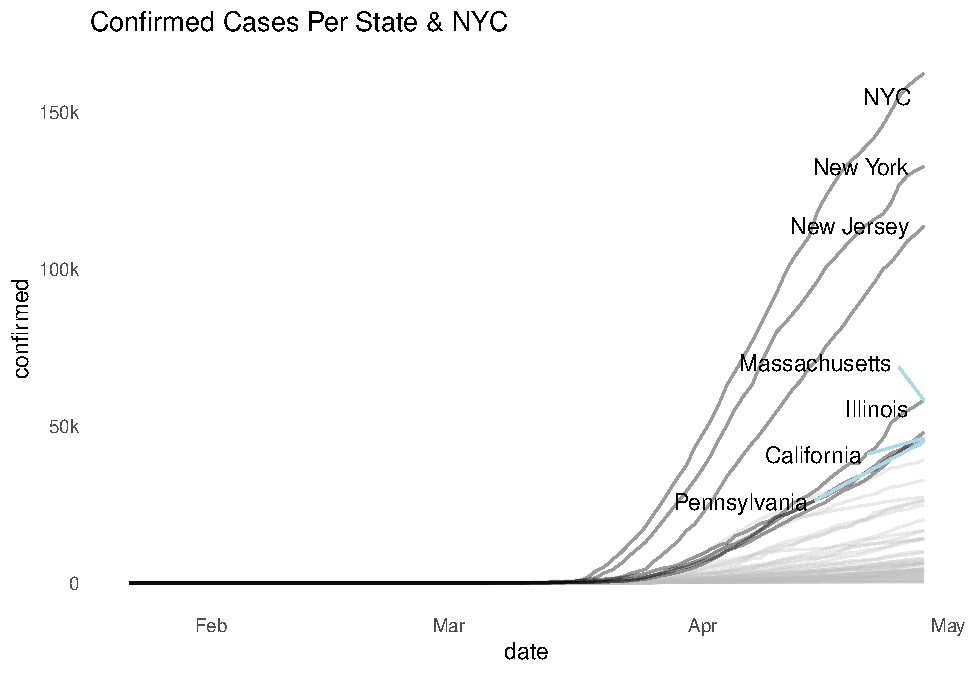
\includegraphics{Project-1---Covid---Final_files/figure-latex/unnamed-chunk-16-1.pdf}

Maybe we should also take a peak at what's going on inside our own
state?

\begin{Shaded}
\begin{Highlighting}[]
\NormalTok{us_data }\OperatorTok
\StringTok{  }\KeywordTok{filter}\NormalTok{(confirm_deaths }\OperatorTok{==}\StringTok{ "confirmed"}\NormalTok{,}
\NormalTok{         province_state }\OperatorTok{==}\StringTok{ "New York"}\NormalTok{)}\OperatorTok
\StringTok{  }\KeywordTok{mutate}\NormalTok{(}\DataTypeTok{province_state =} \KeywordTok{ifelse}\NormalTok{(admin2 }\OperatorTok{==}\StringTok{ "New York"}\NormalTok{, }\StringTok{"NYC"}\NormalTok{, province_state)) }\OperatorTok
\StringTok{  }\KeywordTok{group_by}\NormalTok{(date, province_state,admin2)}\OperatorTok
\StringTok{  }\KeywordTok{summarise}\NormalTok{(}\DataTypeTok{confirmed =} \KeywordTok{sum}\NormalTok{(cum_values)) }\OperatorTok
\KeywordTok{ggplot}\NormalTok{(}\KeywordTok{aes}\NormalTok{(date,confirmed, }\DataTypeTok{group =}\NormalTok{ admin2)) }\OperatorTok{+}
\StringTok{    }\KeywordTok{geom_line}\NormalTok{(}\DataTypeTok{alpha =} \DecValTok{1}\OperatorTok{/}\DecValTok{3}\NormalTok{)}\OperatorTok{+}
\StringTok{    }\KeywordTok{gghighlight}\NormalTok{(}\KeywordTok{max}\NormalTok{(confirmed) }\OperatorTok{>}\StringTok{ }\DecValTok{15000}\NormalTok{,}
            \DataTypeTok{label_params =} \KeywordTok{list}\NormalTok{(}
                \DataTypeTok{fill =} \OtherTok{NA}\NormalTok{,}
                \DataTypeTok{segment.color =} \StringTok{"light blue"}\NormalTok{,}
                \DataTypeTok{label.size =} \OtherTok{NA}
\NormalTok{            )) }\OperatorTok{+}
\StringTok{    }\KeywordTok{scale_y_continuous}\NormalTok{(}\DataTypeTok{labels =}\NormalTok{ addUnits)}\OperatorTok{+}
\StringTok{  }\NormalTok{Eki_theme }\OperatorTok{+}
\StringTok{  }\KeywordTok{ggtitle}\NormalTok{(}\StringTok{"Confirmed Cases in New York Localities"}\NormalTok{)}
\end{Highlighting}
\end{Shaded}

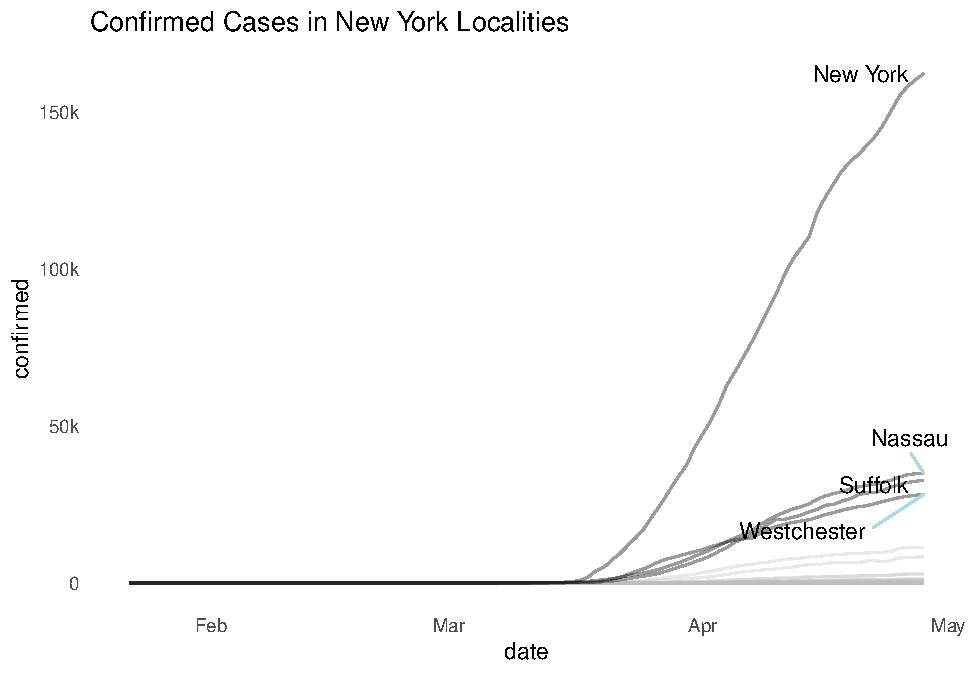
\includegraphics{Project-1---Covid---Final_files/figure-latex/unnamed-chunk-17-1.pdf}

\hypertarget{lets-zoom-in-on-nyc}{%
\subsection{Let's zoom in on NYC}\label{lets-zoom-in-on-nyc}}

Let's get daily additions

\begin{Shaded}
\begin{Highlighting}[]
\NormalTok{foo <-}\StringTok{ }\NormalTok{us_data }\OperatorTok
\StringTok{  }\KeywordTok{filter}\NormalTok{(admin2 }\OperatorTok{==}\StringTok{  "New York"}\NormalTok{,}
\NormalTok{         date }\OperatorTok{>}\StringTok{ "2020-03-01"}\NormalTok{)}\OperatorTok
\StringTok{  }\KeywordTok{group_by}\NormalTok{(confirm_deaths,admin2)}\OperatorTok
\StringTok{  }\KeywordTok{mutate}\NormalTok{(}\DataTypeTok{daily_vals =}\NormalTok{ cum_values }\OperatorTok{-}\StringTok{ }\KeywordTok{lag}\NormalTok{(cum_values))}

\NormalTok{dailyConfirmed_nyc_plot <-}\StringTok{ }\NormalTok{foo }\OperatorTok
\StringTok{  }\KeywordTok{filter}\NormalTok{(confirm_deaths }\OperatorTok{==}\StringTok{ "confirmed"}\NormalTok{) }\OperatorTok
\KeywordTok{ggplot}\NormalTok{(}\KeywordTok{aes}\NormalTok{(}\DataTypeTok{y =}\NormalTok{ daily_vals, }\DataTypeTok{x =}\NormalTok{ date)) }\OperatorTok{+}
\StringTok{  }\KeywordTok{geom_col}\NormalTok{(}\DataTypeTok{width =} \FloatTok{.4}\NormalTok{) }\OperatorTok{+}\StringTok{ }
\StringTok{  }\NormalTok{Eki_theme}\OperatorTok{+}
\StringTok{  }\KeywordTok{scale_y_continuous}\NormalTok{(}\DataTypeTok{labels =}\NormalTok{ addUnits)}\OperatorTok{+}
\StringTok{  }\KeywordTok{ggtitle}\NormalTok{(}\StringTok{"Daily Cases"}\NormalTok{)}\OperatorTok{+}
\StringTok{  }\KeywordTok{ylab}\NormalTok{(}\StringTok{"New Cases"}\NormalTok{)}

\NormalTok{totalConfirmed_nyc_plot <-}\StringTok{ }\NormalTok{foo }\OperatorTok
\StringTok{  }\KeywordTok{filter}\NormalTok{(confirm_deaths }\OperatorTok{==}\StringTok{ "confirmed"}\NormalTok{) }\OperatorTok
\KeywordTok{ggplot}\NormalTok{(}\KeywordTok{aes}\NormalTok{(}\DataTypeTok{y =}\NormalTok{ cum_values, }\DataTypeTok{x =}\NormalTok{ date)) }\OperatorTok{+}
\StringTok{  }\KeywordTok{geom_col}\NormalTok{(}\DataTypeTok{width =} \FloatTok{.4}\NormalTok{) }\OperatorTok{+}\StringTok{ }
\StringTok{  }\NormalTok{Eki_theme}\OperatorTok{+}
\StringTok{  }\KeywordTok{scale_y_continuous}\NormalTok{(}\DataTypeTok{labels =}\NormalTok{ addUnits)}\OperatorTok{+}
\StringTok{  }\KeywordTok{ggtitle}\NormalTok{(}\StringTok{"Total Cases"}\NormalTok{)}\OperatorTok{+}
\StringTok{  }\KeywordTok{ylab}\NormalTok{(}\StringTok{"Cum. Cases"}\NormalTok{)}

\NormalTok{dailyConfirmed_nyc_plot }\OperatorTok{+}\StringTok{ }\NormalTok{totalConfirmed_nyc_plot}
\end{Highlighting}
\end{Shaded}

\begin{verbatim}
## Warning: Removed 1 rows containing missing values (position_stack).
\end{verbatim}

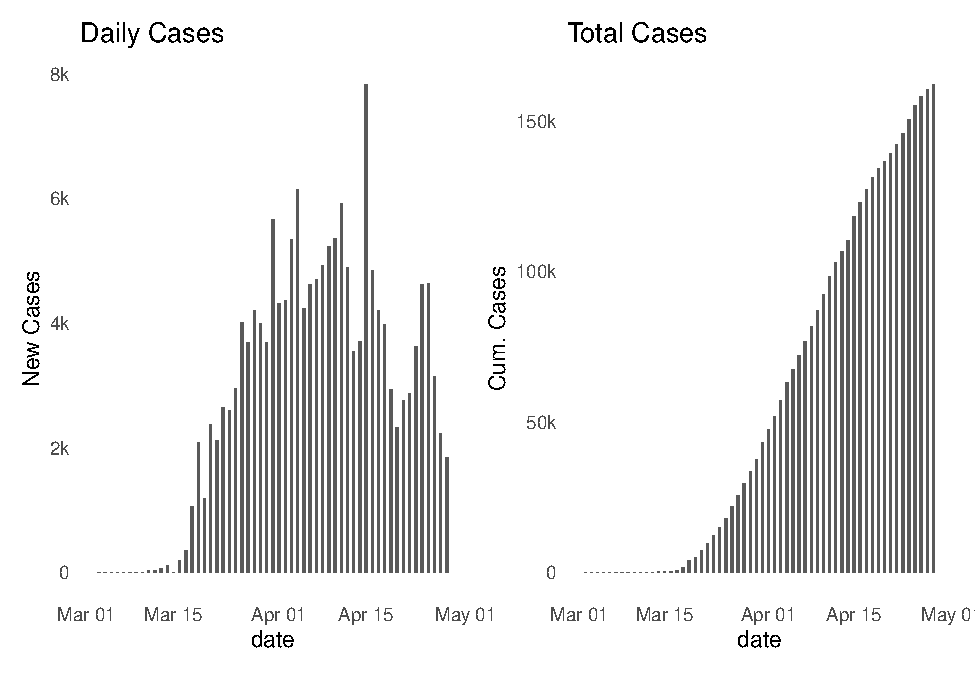
\includegraphics{Project-1---Covid---Final_files/figure-latex/unnamed-chunk-18-1.pdf}

alright, maybe let's take a look at the left chart on a 3 day rolling
average:

\begin{Shaded}
\begin{Highlighting}[]
\NormalTok{dailyConfirmed_nyc_plot_3dayavg <-}\StringTok{ }\NormalTok{foo }\OperatorTok
\StringTok{  }\KeywordTok{filter}\NormalTok{(confirm_deaths }\OperatorTok{==}\StringTok{ "confirmed"}\NormalTok{) }\OperatorTok
\StringTok{ }\KeywordTok{mutate}\NormalTok{(}\DataTypeTok{daily_vals3=}\KeywordTok{rollapply}\NormalTok{(daily_vals,}\DecValTok{3}\NormalTok{,mean,}\DataTypeTok{fill=}\OtherTok{NA}\NormalTok{)) }\OperatorTok
\KeywordTok{ggplot}\NormalTok{(}\KeywordTok{aes}\NormalTok{(}\DataTypeTok{y =}\NormalTok{ daily_vals3, }\DataTypeTok{x =}\NormalTok{ date)) }\OperatorTok{+}
\StringTok{  }\KeywordTok{geom_col}\NormalTok{(}\DataTypeTok{width =} \FloatTok{.4}\NormalTok{) }\OperatorTok{+}\StringTok{ }
\StringTok{  }\NormalTok{Eki_theme}\OperatorTok{+}
\StringTok{  }\KeywordTok{scale_y_continuous}\NormalTok{(}\DataTypeTok{labels =}\NormalTok{ addUnits) }\OperatorTok{+}
\StringTok{  }\KeywordTok{ggtitle}\NormalTok{(}\StringTok{"Daily Cases; 3 day Avg"}\NormalTok{)}\OperatorTok{+}
\StringTok{  }\KeywordTok{ylab}\NormalTok{(}\StringTok{"New Cases"}\NormalTok{)}

\NormalTok{dailyConfirmed_nyc_plot_3dayavg }\OperatorTok{+}\StringTok{ }\NormalTok{totalConfirmed_nyc_plot}
\end{Highlighting}
\end{Shaded}

\begin{verbatim}
## Warning: Removed 3 rows containing missing values (position_stack).
\end{verbatim}

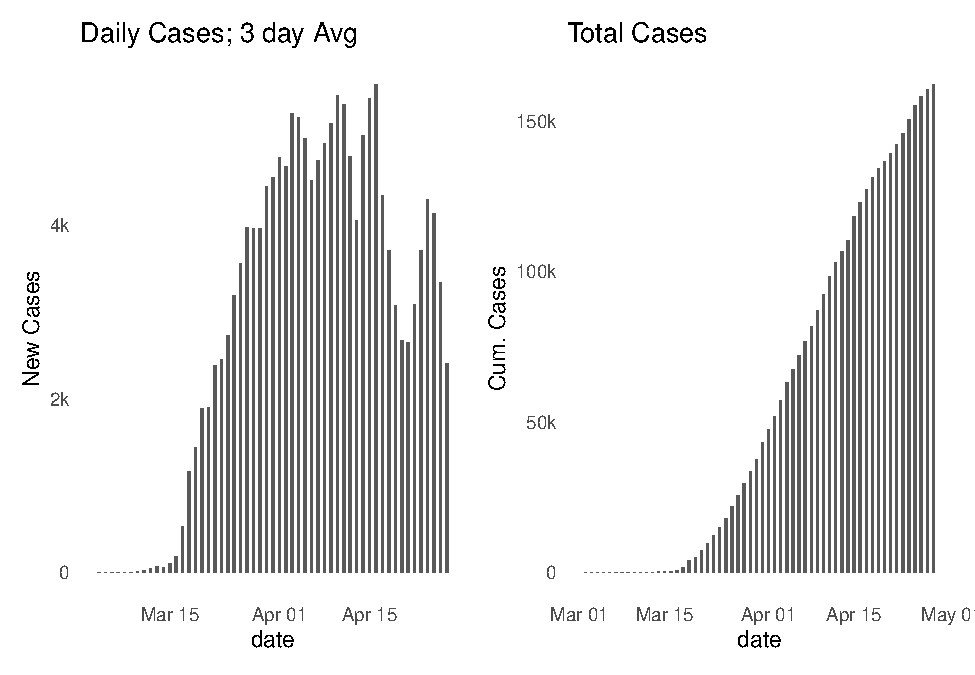
\includegraphics{Project-1---Covid---Final_files/figure-latex/unnamed-chunk-19-1.pdf}

And for deaths, unfortunately.

\begin{Shaded}
\begin{Highlighting}[]
\NormalTok{dailyDeaths_nyc_plot_3dayavg <-}\StringTok{ }\NormalTok{foo }\OperatorTok
\StringTok{  }\KeywordTok{filter}\NormalTok{(confirm_deaths }\OperatorTok{==}\StringTok{ "deaths"}\NormalTok{) }\OperatorTok
\StringTok{ }\KeywordTok{mutate}\NormalTok{(}\DataTypeTok{daily_vals3=}\KeywordTok{rollapply}\NormalTok{(daily_vals,}\DecValTok{3}\NormalTok{,mean,}\DataTypeTok{fill=}\OtherTok{NA}\NormalTok{)) }\OperatorTok
\KeywordTok{ggplot}\NormalTok{(}\KeywordTok{aes}\NormalTok{(}\DataTypeTok{y =}\NormalTok{ daily_vals3, }\DataTypeTok{x =}\NormalTok{ date)) }\OperatorTok{+}
\StringTok{  }\KeywordTok{geom_col}\NormalTok{(}\DataTypeTok{width =} \FloatTok{.4}\NormalTok{) }\OperatorTok{+}\StringTok{ }
\StringTok{  }\NormalTok{Eki_theme}\OperatorTok{+}
\StringTok{  }\KeywordTok{scale_y_continuous}\NormalTok{(}\DataTypeTok{labels =}\NormalTok{ addUnits) }\OperatorTok{+}
\StringTok{  }\KeywordTok{ggtitle}\NormalTok{(}\StringTok{"Daily Deaths; 3 day Avg"}\NormalTok{)}\OperatorTok{+}
\StringTok{  }\KeywordTok{ylab}\NormalTok{(}\StringTok{"New Cases"}\NormalTok{)}

\NormalTok{totalDeaths_nyc_plot <-}\StringTok{ }\NormalTok{foo }\OperatorTok
\StringTok{  }\KeywordTok{filter}\NormalTok{(confirm_deaths }\OperatorTok{==}\StringTok{ "deaths"}\NormalTok{) }\OperatorTok
\KeywordTok{ggplot}\NormalTok{(}\KeywordTok{aes}\NormalTok{(}\DataTypeTok{y =}\NormalTok{ cum_values, }\DataTypeTok{x =}\NormalTok{ date)) }\OperatorTok{+}
\StringTok{  }\KeywordTok{geom_col}\NormalTok{(}\DataTypeTok{width =} \FloatTok{.4}\NormalTok{)}\OperatorTok{+}
\StringTok{  }\NormalTok{Eki_theme}\OperatorTok{+}
\StringTok{  }\KeywordTok{scale_y_continuous}\NormalTok{(}\DataTypeTok{labels =}\NormalTok{ addUnits) }\OperatorTok{+}
\StringTok{  }\KeywordTok{ggtitle}\NormalTok{(}\StringTok{"Total Deaths"}\NormalTok{)}\OperatorTok{+}
\StringTok{  }\KeywordTok{ylab}\NormalTok{(}\StringTok{"Cum. Cases"}\NormalTok{)}

\NormalTok{dailyDeaths_nyc_plot_3dayavg }\OperatorTok{+}\StringTok{ }\NormalTok{totalDeaths_nyc_plot}
\end{Highlighting}
\end{Shaded}

\begin{verbatim}
## Warning: Removed 3 rows containing missing values (position_stack).
\end{verbatim}

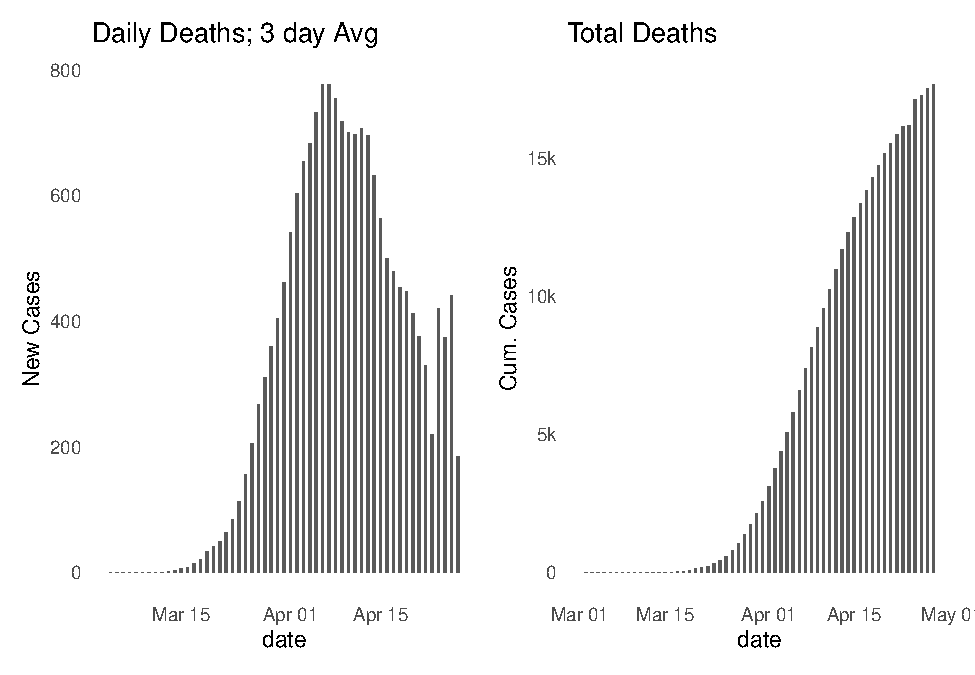
\includegraphics{Project-1---Covid---Final_files/figure-latex/unnamed-chunk-20-1.pdf}

\hypertarget{lets-try-something-fun}{%
\subsection{Let's try something fun}\label{lets-try-something-fun}}

So, yes, I understand this isn't the best ``use case'' for this but I
don't care I'm having fun.

\begin{Shaded}
\begin{Highlighting}[]
\NormalTok{us_data <-}\StringTok{ }\NormalTok{us_data }\OperatorTok
\StringTok{  }\KeywordTok{mutate}\NormalTok{(}\DataTypeTok{combined_key=} \KeywordTok{gsub}\NormalTok{(}\StringTok{", US"}\NormalTok{,}\StringTok{""}\NormalTok{,combined_key))}
\end{Highlighting}
\end{Shaded}

\begin{Shaded}
\begin{Highlighting}[]
\NormalTok{all_locals <-}\StringTok{ }\NormalTok{us_data }\OperatorTok\StringTok{ }
\KeywordTok{filter}\NormalTok{(confirm_deaths }\OperatorTok{==}\StringTok{ "confirmed"}\NormalTok{) }\OperatorTok

\StringTok{  }\KeywordTok{ggplot}\NormalTok{(}\KeywordTok{aes}\NormalTok{(date, cum_values, }\DataTypeTok{group =}\NormalTok{ combined_key)) }\OperatorTok{+}
\StringTok{    }\KeywordTok{geom_line}\NormalTok{(}\DataTypeTok{alpha =} \DecValTok{1}\OperatorTok{/}\DecValTok{3}\NormalTok{) }\OperatorTok{+}
\StringTok{  }\KeywordTok{gghighlight}\NormalTok{(}\KeywordTok{max}\NormalTok{(cum_values) }\OperatorTok{>}\StringTok{ }\DecValTok{20000}\NormalTok{,}
            \DataTypeTok{label_params =} \KeywordTok{list}\NormalTok{(}
                \DataTypeTok{fill =} \OtherTok{NA}\NormalTok{,}
                \DataTypeTok{segment.color =} \StringTok{"light blue"}\NormalTok{,}
                \DataTypeTok{label.size =} \OtherTok{NA}
\NormalTok{            )) }\OperatorTok{+}
\StringTok{  }\KeywordTok{scale_y_continuous}\NormalTok{(}\DataTypeTok{labels =}\NormalTok{ addUnits)}\OperatorTok{+}
\StringTok{  }\NormalTok{Eki_theme }\OperatorTok{+}
\StringTok{  }\KeywordTok{ggtitle}\NormalTok{(}\StringTok{"Confirmed Cases all Localities"}\NormalTok{)}
\end{Highlighting}
\end{Shaded}

\begin{verbatim}
## label_key: combined_key
\end{verbatim}

\begin{Shaded}
\begin{Highlighting}[]
\NormalTok{all_locals_subNYC <-}\StringTok{ }\NormalTok{us_data }\OperatorTok\StringTok{ }
\KeywordTok{filter}\NormalTok{(confirm_deaths }\OperatorTok{==}\StringTok{ "confirmed"}\NormalTok{,}
\NormalTok{       combined_key }\OperatorTok{!=}\StringTok{ "New York City, New York"}\NormalTok{) }\OperatorTok

\StringTok{  }\KeywordTok{ggplot}\NormalTok{(}\KeywordTok{aes}\NormalTok{(date, cum_values, }\DataTypeTok{group =}\NormalTok{ combined_key)) }\OperatorTok{+}
\StringTok{    }\KeywordTok{geom_line}\NormalTok{(}\DataTypeTok{alpha =} \DecValTok{1}\OperatorTok{/}\DecValTok{3}\NormalTok{) }\OperatorTok{+}
\StringTok{  }\KeywordTok{gghighlight}\NormalTok{(}\KeywordTok{max}\NormalTok{(cum_values) }\OperatorTok{>}\StringTok{ }\DecValTok{12000}\NormalTok{,}
            \DataTypeTok{label_params =} \KeywordTok{list}\NormalTok{(}
                \DataTypeTok{fill =} \OtherTok{NA}\NormalTok{,}
                \DataTypeTok{segment.color =} \StringTok{"light blue"}\NormalTok{,}
                \DataTypeTok{label.size =} \OtherTok{NA}\NormalTok{,}
                \DataTypeTok{size =}\DecValTok{2}
\NormalTok{            ))  }\OperatorTok{+}
\StringTok{  }\KeywordTok{scale_y_continuous}\NormalTok{(}\DataTypeTok{labels =}\NormalTok{ addUnits)}\OperatorTok{+}
\StringTok{  }\NormalTok{Eki_theme }\OperatorTok{+}
\StringTok{  }\KeywordTok{ggtitle}\NormalTok{(}\StringTok{"Confirmed Cases all Localities Sub NYC"}\NormalTok{)}
\end{Highlighting}
\end{Shaded}

\begin{verbatim}
## label_key: combined_key
\end{verbatim}

\begin{Shaded}
\begin{Highlighting}[]
\NormalTok{all_locals }\OperatorTok{+}\StringTok{ }\NormalTok{all_locals_subNYC}
\end{Highlighting}
\end{Shaded}

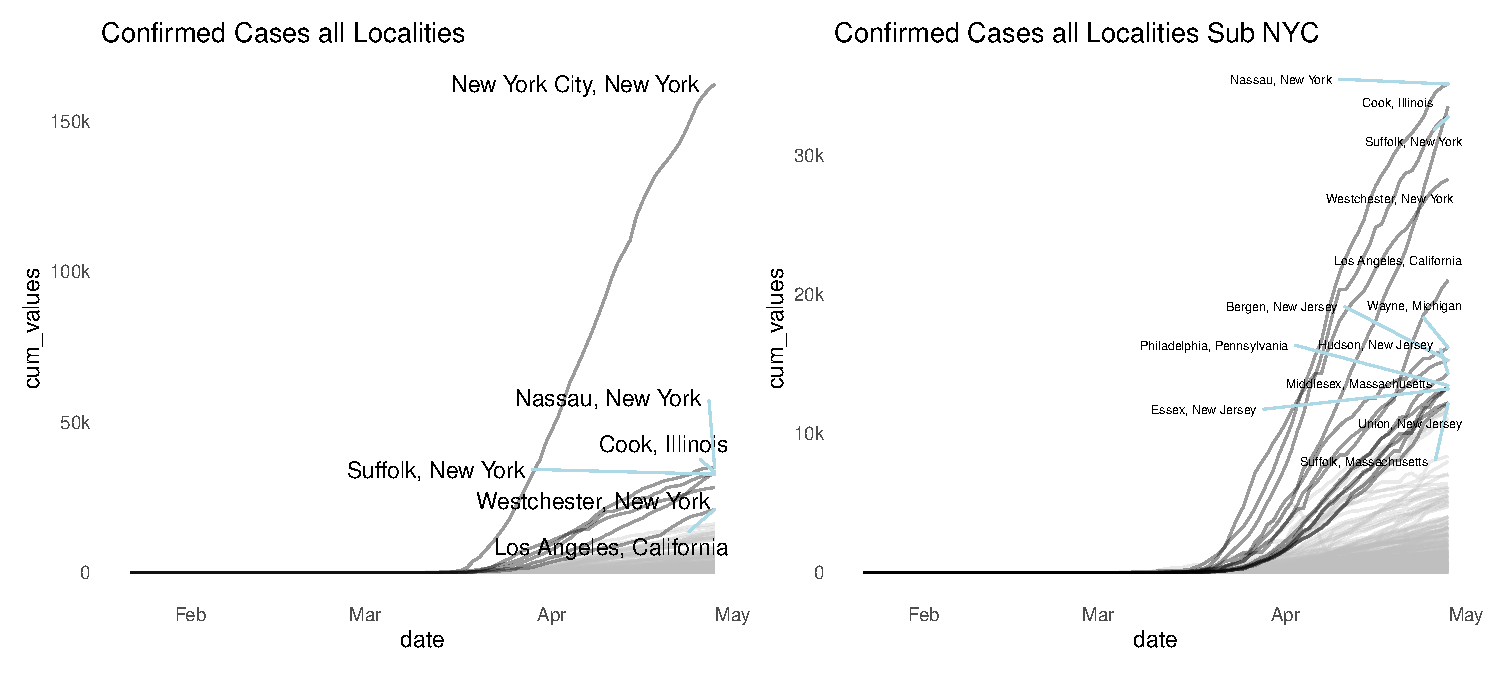
\includegraphics{Project-1---Covid---Final_files/figure-latex/unnamed-chunk-22-1.pdf}

So let's try and fit a small model for deaths based off of days and
confirmed cases:

\begin{Shaded}
\begin{Highlighting}[]
\NormalTok{Suffolk_data <-}\StringTok{ }\NormalTok{us_data }\OperatorTok
\StringTok{    }\KeywordTok{filter}\NormalTok{(combined_key }\OperatorTok{==}\StringTok{ "Suffolk, New York"}\NormalTok{,}
\NormalTok{           date }\OperatorTok{>=}\StringTok{ "2020-03-01"}\NormalTok{)}\OperatorTok
\StringTok{    }\KeywordTok{pivot_wider}\NormalTok{(}\DataTypeTok{names_from =}\NormalTok{ confirm_deaths, }\DataTypeTok{values_from =}\NormalTok{ cum_values)}\OperatorTok
\StringTok{      }\KeywordTok{group_by}\NormalTok{(combined_key)}\OperatorTok
\StringTok{    }\KeywordTok{mutate}\NormalTok{(}
        \DataTypeTok{daily_deaths =}\NormalTok{ deaths }\OperatorTok{-}\StringTok{ }\KeywordTok{lag}\NormalTok{(deaths),}
        \DataTypeTok{daily_deaths3=}\KeywordTok{rollapply}\NormalTok{(daily_deaths,}\DecValTok{3}\NormalTok{,mean,}\DataTypeTok{fill=}\DecValTok{0}\NormalTok{),}
       
        \DataTypeTok{daily_confirmed =}\NormalTok{ confirmed }\OperatorTok{-}\StringTok{ }\KeywordTok{lag}\NormalTok{(confirmed),}
        \DataTypeTok{daily_confirmed3=}\KeywordTok{rollapply}\NormalTok{(daily_confirmed,}\DecValTok{3}\NormalTok{,mean,}\DataTypeTok{fill=}\DecValTok{0}\NormalTok{))}\OperatorTok
\StringTok{    }\KeywordTok{replace_na}\NormalTok{(}\KeywordTok{list}\NormalTok{(}\DataTypeTok{daily_deaths3 =} \DecValTok{0}\NormalTok{, }\DataTypeTok{daily_confirmed3 =} \DecValTok{0}\NormalTok{, }\DataTypeTok{daily_deaths =}\DecValTok{0}\NormalTok{, }\DataTypeTok{daily_confirmed =} \DecValTok{0}\NormalTok{))}
\end{Highlighting}
\end{Shaded}

So, Let's fit a model to one of the localities and see how things look.

\begin{Shaded}
\begin{Highlighting}[]
\NormalTok{suf_mod <-}\StringTok{ }\KeywordTok{lm}\NormalTok{(daily_deaths3 }\OperatorTok{~}\StringTok{ }\NormalTok{daily_confirmed3 }\OperatorTok{+}\StringTok{ }\NormalTok{date, }\DataTypeTok{data =}\NormalTok{ Suffolk_data)}
\end{Highlighting}
\end{Shaded}

\begin{Shaded}
\begin{Highlighting}[]
\NormalTok{Pure_data <-}\StringTok{ }\NormalTok{Suffolk_data }\OperatorTok
\StringTok{    }\KeywordTok{ggplot}\NormalTok{(}\KeywordTok{aes}\NormalTok{(date, daily_deaths3))}\OperatorTok{+}
\StringTok{    }\KeywordTok{geom_line}\NormalTok{()}\OperatorTok{+}
\StringTok{    }\KeywordTok{ggtitle}\NormalTok{(}\StringTok{"Suffolk Deaths"}\NormalTok{)}

\NormalTok{LinTrendPlot <-}\StringTok{ }\NormalTok{Suffolk_data }\OperatorTok\StringTok{ }
\StringTok{  }\KeywordTok{add_predictions}\NormalTok{(suf_mod) }\OperatorTok
\StringTok{  }\KeywordTok{ggplot}\NormalTok{(}\KeywordTok{aes}\NormalTok{(date, pred)) }\OperatorTok{+}\StringTok{ }
\StringTok{  }\KeywordTok{geom_line}\NormalTok{() }\OperatorTok{+}\StringTok{ }
\StringTok{  }\KeywordTok{ggtitle}\NormalTok{(}\StringTok{"Linear trend + "}\NormalTok{)}

\NormalTok{residLine <-}\StringTok{ }\NormalTok{Suffolk_data }\OperatorTok\StringTok{ }
\StringTok{  }\KeywordTok{add_residuals}\NormalTok{(suf_mod) }\OperatorTok\StringTok{ }
\StringTok{  }\KeywordTok{ggplot}\NormalTok{(}\KeywordTok{aes}\NormalTok{(date, resid)) }\OperatorTok{+}\StringTok{ }
\StringTok{  }\KeywordTok{geom_hline}\NormalTok{(}\DataTypeTok{yintercept =} \DecValTok{0}\NormalTok{, }\DataTypeTok{colour =} \StringTok{"grey"}\NormalTok{, }\DataTypeTok{size =} \DecValTok{3}\NormalTok{) }\OperatorTok{+}\StringTok{ }
\StringTok{  }\KeywordTok{geom_line}\NormalTok{() }\OperatorTok{+}\StringTok{ }
\StringTok{  }\KeywordTok{ggtitle}\NormalTok{(}\StringTok{"Remaining pattern"}\NormalTok{)}\OperatorTok{+}
\StringTok{    }\NormalTok{Eki_theme}

\NormalTok{Pure_data }\OperatorTok{/}\StringTok{ }\NormalTok{LinTrendPlot }\OperatorTok{/}\StringTok{ }\NormalTok{residLine}
\end{Highlighting}
\end{Shaded}

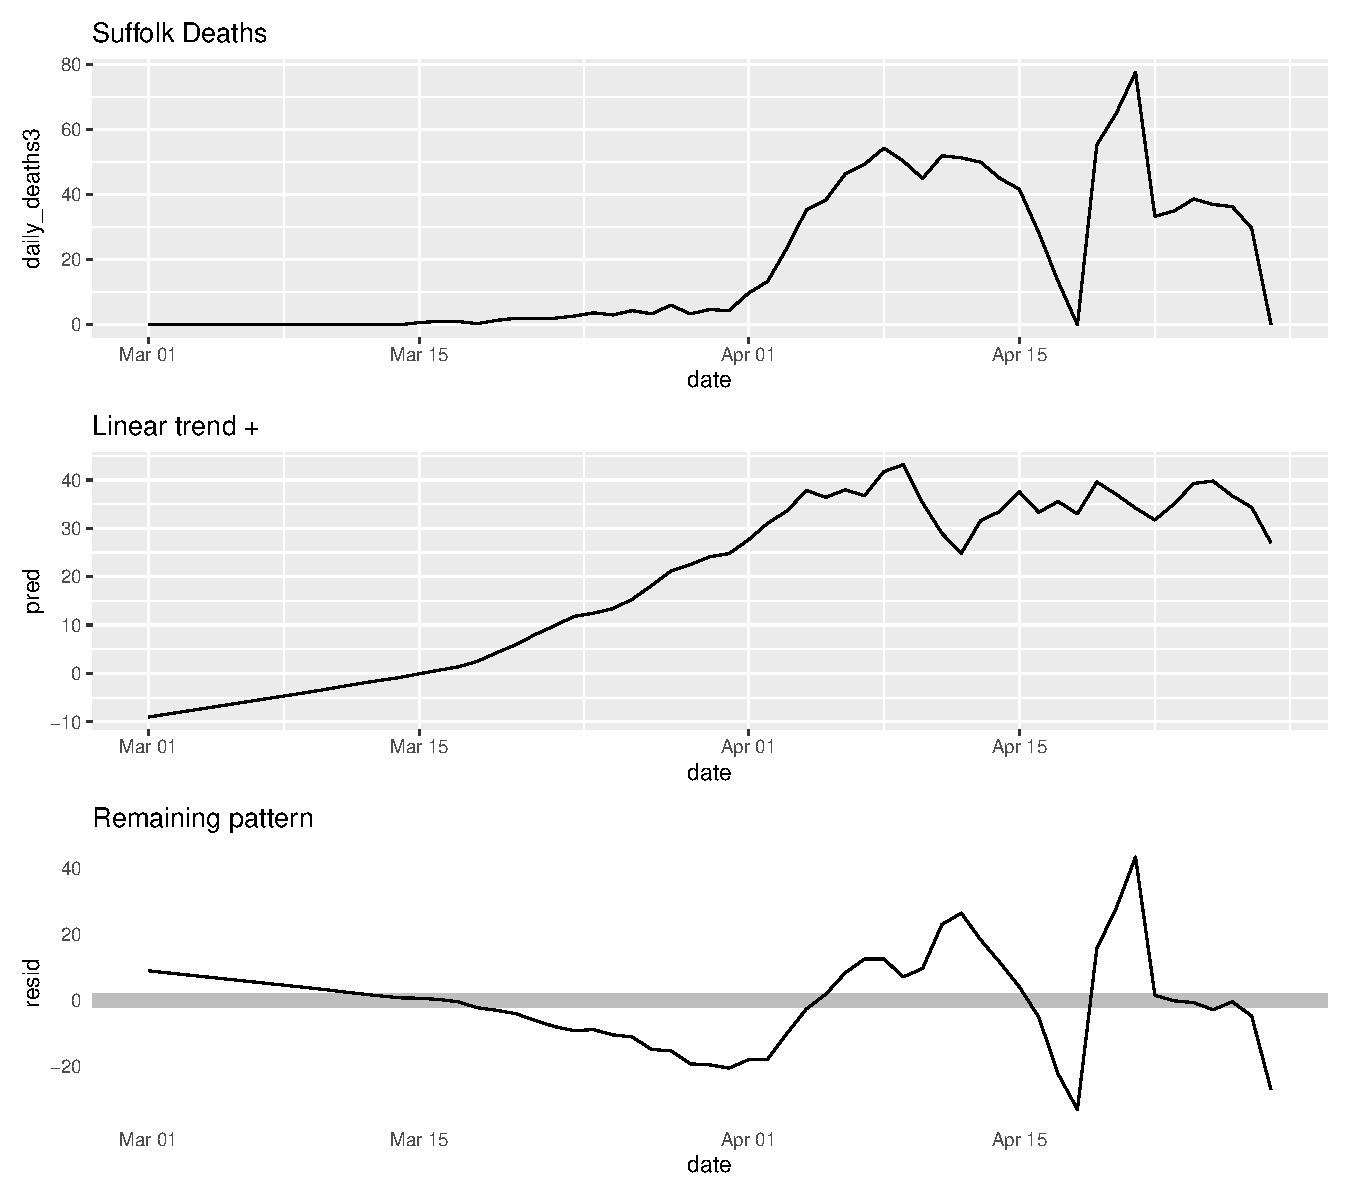
\includegraphics{Project-1---Covid---Final_files/figure-latex/unnamed-chunk-25-1.pdf}

So let's group our data into a nested dataframe so we can fit a model on
every locality.

\begin{Shaded}
\begin{Highlighting}[]
\NormalTok{us_step1 <-}\StringTok{ }\NormalTok{us_data }\OperatorTok
\StringTok{    }\KeywordTok{select}\NormalTok{(admin2, combined_key, date, province_state, population, }
\NormalTok{           confirm_deaths, cum_values)}\OperatorTok
\StringTok{    }\KeywordTok{pivot_wider}\NormalTok{(}\DataTypeTok{names_from =}\NormalTok{ confirm_deaths, }\DataTypeTok{values_from =}\NormalTok{ cum_values)}\OperatorTok\StringTok{     }\KeywordTok{group_by}\NormalTok{(combined_key)}\OperatorTok
\StringTok{    }\KeywordTok{mutate}\NormalTok{(}
        \DataTypeTok{daily_deaths =}\NormalTok{ deaths }\OperatorTok{-}\StringTok{ }\KeywordTok{lag}\NormalTok{(deaths),}
        \DataTypeTok{daily_deaths3=}\KeywordTok{rollapply}\NormalTok{(daily_deaths,}\DecValTok{3}\NormalTok{,mean,}\DataTypeTok{fill=}\DecValTok{0}\NormalTok{),}
       
        \DataTypeTok{daily_confirmed =}\NormalTok{ confirmed }\OperatorTok{-}\StringTok{ }\KeywordTok{lag}\NormalTok{(confirmed),}
        \DataTypeTok{daily_confirmed3=}\KeywordTok{rollapply}\NormalTok{(daily_confirmed,}\DecValTok{3}\NormalTok{,mean,}\DataTypeTok{fill=}\DecValTok{0}\NormalTok{))}\OperatorTok
\StringTok{    }\KeywordTok{replace_na}\NormalTok{(}\KeywordTok{list}\NormalTok{(}\DataTypeTok{daily_deaths3 =} \DecValTok{0}\NormalTok{, }\DataTypeTok{daily_confirmed3 =} \DecValTok{0}\NormalTok{, }\DataTypeTok{daily_deaths =}\DecValTok{0}\NormalTok{, }\DataTypeTok{daily_confirmed =} \DecValTok{0}\NormalTok{))}
    
\NormalTok{byLocality <-}\StringTok{ }\NormalTok{us_step1 }\OperatorTok
\StringTok{    }\KeywordTok{group_by}\NormalTok{(combined_key) }\OperatorTok
\StringTok{    }\KeywordTok{nest}\NormalTok{()}
    
\NormalTok{byLocality}
\end{Highlighting}
\end{Shaded}

\begin{verbatim}
## # A tibble: 3,262 x 2
## # Groups:   combined_key [3,262]
##    combined_key             data              
##    <chr>                    <list>            
##  1 American Samoa           <tibble [98 x 10]>
##  2 Guam                     <tibble [98 x 10]>
##  3 Northern Mariana Islands <tibble [98 x 10]>
##  4 Puerto Rico              <tibble [98 x 10]>
##  5 Virgin Islands           <tibble [98 x 10]>
##  6 Autauga, Alabama         <tibble [98 x 10]>
##  7 Baldwin, Alabama         <tibble [98 x 10]>
##  8 Barbour, Alabama         <tibble [98 x 10]>
##  9 Bibb, Alabama            <tibble [98 x 10]>
## 10 Blount, Alabama          <tibble [98 x 10]>
## # ... with 3,252 more rows
\end{verbatim}

It's not very easy to look into this on an aggregate scale - but you can
still peek.

\begin{Shaded}
\begin{Highlighting}[]
\NormalTok{byLocality}\OperatorTok{$}\NormalTok{data[[}\DecValTok{5}\NormalTok{]]}
\end{Highlighting}
\end{Shaded}

\begin{verbatim}
## # A tibble: 98 x 10
##    admin2 date       province_state population deaths confirmed daily_deaths
##    <chr>  <date>     <chr>               <dbl>  <dbl>     <dbl>        <dbl>
##  1 <NA>   2020-01-22 Virgin Islands     107268      0         0            0
##  2 <NA>   2020-01-23 Virgin Islands     107268      0         0            0
##  3 <NA>   2020-01-24 Virgin Islands     107268      0         0            0
##  4 <NA>   2020-01-25 Virgin Islands     107268      0         0            0
##  5 <NA>   2020-01-26 Virgin Islands     107268      0         0            0
##  6 <NA>   2020-01-27 Virgin Islands     107268      0         0            0
##  7 <NA>   2020-01-28 Virgin Islands     107268      0         0            0
##  8 <NA>   2020-01-29 Virgin Islands     107268      0         0            0
##  9 <NA>   2020-01-30 Virgin Islands     107268      0         0            0
## 10 <NA>   2020-01-31 Virgin Islands     107268      0         0            0
## # ... with 88 more rows, and 3 more variables: daily_deaths3 <dbl>,
## #   daily_confirmed <dbl>, daily_confirmed3 <dbl>
\end{verbatim}

Alright, so now we have the data ready for this test, let's get our
tools to actually perform it ready.

\begin{Shaded}
\begin{Highlighting}[]
\NormalTok{local_model <-}\StringTok{ }\ControlFlowTok{function}\NormalTok{(df) \{}
    \KeywordTok{lm}\NormalTok{(daily_deaths3 }\OperatorTok{~}\StringTok{ }\NormalTok{daily_confirmed3 }\OperatorTok{+}\StringTok{ }\NormalTok{date, }\DataTypeTok{data =}\NormalTok{ df)}
\NormalTok{\}}
\end{Highlighting}
\end{Shaded}

The dataframes are in a list so we can use purrr's map() to apply our
function to each element. Purrr is kind of a scary package for me tbh.

\begin{Shaded}
\begin{Highlighting}[]
\NormalTok{byLocality <-}\StringTok{ }\NormalTok{byLocality }\OperatorTok
\StringTok{    }\KeywordTok{mutate}\NormalTok{(}\DataTypeTok{model =} \KeywordTok{map}\NormalTok{(data, local_model))}
\end{Highlighting}
\end{Shaded}

We did it this way to keep the results and data tied together and avoid
errors.

\begin{Shaded}
\begin{Highlighting}[]
\NormalTok{byLocality}
\end{Highlighting}
\end{Shaded}

\begin{verbatim}
## # A tibble: 3,262 x 3
## # Groups:   combined_key [3,262]
##    combined_key             data               model 
##    <chr>                    <list>             <list>
##  1 American Samoa           <tibble [98 x 10]> <lm>  
##  2 Guam                     <tibble [98 x 10]> <lm>  
##  3 Northern Mariana Islands <tibble [98 x 10]> <lm>  
##  4 Puerto Rico              <tibble [98 x 10]> <lm>  
##  5 Virgin Islands           <tibble [98 x 10]> <lm>  
##  6 Autauga, Alabama         <tibble [98 x 10]> <lm>  
##  7 Baldwin, Alabama         <tibble [98 x 10]> <lm>  
##  8 Barbour, Alabama         <tibble [98 x 10]> <lm>  
##  9 Bibb, Alabama            <tibble [98 x 10]> <lm>  
## 10 Blount, Alabama          <tibble [98 x 10]> <lm>  
## # ... with 3,252 more rows
\end{verbatim}

Add residuals

\begin{Shaded}
\begin{Highlighting}[]
\NormalTok{byLocality <-}\StringTok{ }\NormalTok{byLocality }\OperatorTok\StringTok{ }
\StringTok{  }\KeywordTok{mutate}\NormalTok{(}
    \DataTypeTok{resids =} \KeywordTok{map2}\NormalTok{(data, model, add_residuals)}
\NormalTok{  )}
\end{Highlighting}
\end{Shaded}

Unnest stem.

\begin{Shaded}
\begin{Highlighting}[]
\NormalTok{resids <-}\StringTok{ }\KeywordTok{unnest}\NormalTok{(byLocality, resids)}
\end{Highlighting}
\end{Shaded}

\begin{Shaded}
\begin{Highlighting}[]
\NormalTok{resids}
\end{Highlighting}
\end{Shaded}

\begin{verbatim}
## # A tibble: 319,676 x 14
## # Groups:   combined_key [3,262]
##    combined_key data  model admin2 date       province_state population deaths
##    <chr>        <lis> <lis> <chr>  <date>     <chr>               <dbl>  <dbl>
##  1 American Sa~ <tib~ <lm>  <NA>   2020-01-22 American Samoa      55641      0
##  2 American Sa~ <tib~ <lm>  <NA>   2020-01-23 American Samoa      55641      0
##  3 American Sa~ <tib~ <lm>  <NA>   2020-01-24 American Samoa      55641      0
##  4 American Sa~ <tib~ <lm>  <NA>   2020-01-25 American Samoa      55641      0
##  5 American Sa~ <tib~ <lm>  <NA>   2020-01-26 American Samoa      55641      0
##  6 American Sa~ <tib~ <lm>  <NA>   2020-01-27 American Samoa      55641      0
##  7 American Sa~ <tib~ <lm>  <NA>   2020-01-28 American Samoa      55641      0
##  8 American Sa~ <tib~ <lm>  <NA>   2020-01-29 American Samoa      55641      0
##  9 American Sa~ <tib~ <lm>  <NA>   2020-01-30 American Samoa      55641      0
## 10 American Sa~ <tib~ <lm>  <NA>   2020-01-31 American Samoa      55641      0
## # ... with 319,666 more rows, and 6 more variables: confirmed <dbl>,
## #   daily_deaths <dbl>, daily_deaths3 <dbl>, daily_confirmed <dbl>,
## #   daily_confirmed3 <dbl>, resid <dbl>
\end{verbatim}

\begin{Shaded}
\begin{Highlighting}[]
\NormalTok{residualPlot <-}\StringTok{ }\NormalTok{resids }\OperatorTok
\StringTok{  }\KeywordTok{ggplot}\NormalTok{(}\KeywordTok{aes}\NormalTok{(date, resid)) }\OperatorTok{+}
\StringTok{    }\KeywordTok{geom_line}\NormalTok{(}\KeywordTok{aes}\NormalTok{(}\DataTypeTok{group =}\NormalTok{ combined_key), }\DataTypeTok{alpha =} \DecValTok{1} \OperatorTok{/}\StringTok{ }\DecValTok{3}\NormalTok{) }\OperatorTok{+}
\StringTok{    }\KeywordTok{geom_smooth}\NormalTok{(}\DataTypeTok{se =} \OtherTok{FALSE}\NormalTok{)}\OperatorTok{+}
\StringTok{    }\NormalTok{Eki_theme}


\NormalTok{residualPlot}
\end{Highlighting}
\end{Shaded}

\begin{verbatim}
## `geom_smooth()` using method = 'gam' and formula 'y ~ s(x, bs = "cs")'
\end{verbatim}

\includegraphics{Project-1---Covid---Final_files/figure-latex/unnamed-chunk-34-1.pdf}

\begin{Shaded}
\begin{Highlighting}[]
\CommentTok{# build our categories - could do a join but I don't want to have to share additional data}
\NormalTok{northeast <-}\StringTok{ }\KeywordTok{c}\NormalTok{(}\StringTok{"Connecticut"}\NormalTok{, }\StringTok{"Maine"}\NormalTok{, }\StringTok{"Massachusetts"}\NormalTok{, }\StringTok{"New Hampshire"}\NormalTok{, }\StringTok{"Rhode Island"}\NormalTok{, }\StringTok{"Vermont"}\NormalTok{, }\StringTok{"New Jersey"}\NormalTok{, }\StringTok{"New York"}\NormalTok{, }\StringTok{"Pennsylvania"}\NormalTok{)}

\NormalTok{midwest <-}\StringTok{ }\KeywordTok{c}\NormalTok{(}\StringTok{"Illinois"}\NormalTok{, }\StringTok{"Indiana"}\NormalTok{, }\StringTok{"Michigan"}\NormalTok{, }\StringTok{"Ohio"}\NormalTok{, }\StringTok{"Wisconsin"}\NormalTok{, }\StringTok{"Iowa"}\NormalTok{, }\StringTok{"Kansas"}\NormalTok{, }\StringTok{"Minnesota"}\NormalTok{, }\StringTok{"Missouri"}\NormalTok{, }\StringTok{"Nebraska"}\NormalTok{, }\StringTok{"North Dakota"}\NormalTok{, }\StringTok{"South Dakota"}\NormalTok{)}

\NormalTok{south <-}\StringTok{ }\KeywordTok{c}\NormalTok{(}\StringTok{"Delaware"}\NormalTok{, }\StringTok{"Florida"}\NormalTok{, }\StringTok{"Georgia"}\NormalTok{, }\StringTok{"Maryland"}\NormalTok{, }\StringTok{"North Carolina"}\NormalTok{, }\StringTok{"South Carolina"}\NormalTok{, }\StringTok{"Virginia"}\NormalTok{, }\StringTok{"District of Columbia"}\NormalTok{, }\StringTok{"West Virginia"}\NormalTok{, }\StringTok{"Alabama"}\NormalTok{, }\StringTok{"Kentucky"}\NormalTok{, }\StringTok{"Mississippi"}\NormalTok{, }\StringTok{"Tennessee"}\NormalTok{, }\StringTok{"Arkansas"}\NormalTok{, }\StringTok{"Louisiana"}\NormalTok{, }\StringTok{"Oklahoma"}\NormalTok{, }\StringTok{"Texas"}\NormalTok{)}

\NormalTok{west <-}\StringTok{ }\KeywordTok{c}\NormalTok{(}\StringTok{"Arizona"}\NormalTok{, }\StringTok{"Colorado"}\NormalTok{, }\StringTok{"Idaho"}\NormalTok{, }\StringTok{"Montana"}\NormalTok{, }\StringTok{"Nevada"}\NormalTok{, }\StringTok{"New Mexico"}\NormalTok{, }\StringTok{"Utah"}\NormalTok{, }\StringTok{"Wyoming"}\NormalTok{, }\StringTok{"Alaska"}\NormalTok{, }\StringTok{"California"}\NormalTok{, }\StringTok{"Hawaii"}\NormalTok{, }\StringTok{"Oregon"}\NormalTok{, }\StringTok{"Washington"}\NormalTok{)}

\CommentTok{#add those regions}

\NormalTok{resids}\OperatorTok{$}\NormalTok{region <-}\StringTok{ }\KeywordTok{case_when}\NormalTok{(}
\NormalTok{    resids}\OperatorTok{$}\NormalTok{province_state }\OperatorTok\StringTok{ }\NormalTok{northeast }\OperatorTok{~}\StringTok{ "northeast"}\NormalTok{,}
\NormalTok{    resids}\OperatorTok{$}\NormalTok{province_state }\OperatorTok\StringTok{ }\NormalTok{midwest }\OperatorTok{~}\StringTok{ "midwest"}\NormalTok{,}
\NormalTok{    resids}\OperatorTok{$}\NormalTok{province_state }\OperatorTok\StringTok{ }\NormalTok{south }\OperatorTok{~}\StringTok{ "south"}\NormalTok{,}
\NormalTok{    resids}\OperatorTok{$}\NormalTok{province_state }\OperatorTok\StringTok{ }\NormalTok{west }\OperatorTok{~}\StringTok{ "west"}\NormalTok{,}
    \OtherTok{TRUE} \OperatorTok{~}\StringTok{ "other"}
\NormalTok{)}
\end{Highlighting}
\end{Shaded}

\begin{Shaded}
\begin{Highlighting}[]
\NormalTok{ resids }\OperatorTok
\StringTok{  }\KeywordTok{ggplot}\NormalTok{(}\KeywordTok{aes}\NormalTok{(date, resid)) }\OperatorTok{+}
\StringTok{    }\KeywordTok{geom_line}\NormalTok{(}\KeywordTok{aes}\NormalTok{(}\DataTypeTok{group =}\NormalTok{ combined_key), }\DataTypeTok{alpha =} \DecValTok{1} \OperatorTok{/}\StringTok{ }\DecValTok{3}\NormalTok{) }\OperatorTok{+}
\StringTok{    }\KeywordTok{geom_smooth}\NormalTok{(}\DataTypeTok{se =} \OtherTok{FALSE}\NormalTok{)}\OperatorTok{+}
\StringTok{    }\NormalTok{Eki_theme }\OperatorTok{+}
\StringTok{    }\KeywordTok{facet_wrap}\NormalTok{(}\OperatorTok{~}\NormalTok{region,}
               \DataTypeTok{scales =} \StringTok{"free_y"}\NormalTok{)}
\end{Highlighting}
\end{Shaded}

\begin{verbatim}
## Warning: namespace 'plyr' is not available and has been replaced
## by .GlobalEnv when processing object 'collapse'
\end{verbatim}

\begin{verbatim}
## `geom_smooth()` using method = 'gam' and formula 'y ~ s(x, bs = "cs")'
\end{verbatim}

\includegraphics{Project-1---Covid---Final_files/figure-latex/unnamed-chunk-36-1.pdf}

Dope, great models doing the worst in the most important area. Well if
it was this easy\ldots.

\begin{Shaded}
\begin{Highlighting}[]
\KeywordTok{library}\NormalTok{(broom)}
\end{Highlighting}
\end{Shaded}

\begin{verbatim}
## 
## Attaching package: 'broom'
\end{verbatim}

\begin{verbatim}
## The following object is masked from 'package:modelr':
## 
##     bootstrap
\end{verbatim}

\begin{Shaded}
\begin{Highlighting}[]
\NormalTok{broom}\OperatorTok{::}\KeywordTok{glance}\NormalTok{(suf_mod)}
\end{Highlighting}
\end{Shaded}

\begin{verbatim}
## # A tibble: 1 x 11
##   r.squared adj.r.squared sigma statistic  p.value    df logLik   AIC   BIC
##       <dbl>         <dbl> <dbl>     <dbl>    <dbl> <int>  <dbl> <dbl> <dbl>
## 1     0.620         0.606  13.9      45.7 1.71e-12     3  -238.  483.  491.
## # ... with 2 more variables: deviance <dbl>, df.residual <int>
\end{verbatim}

\begin{Shaded}
\begin{Highlighting}[]
\NormalTok{model_deets <-}\StringTok{ }\NormalTok{byLocality }\OperatorTok\StringTok{ }
\StringTok{  }\KeywordTok{mutate}\NormalTok{(}\DataTypeTok{glance =} \KeywordTok{map}\NormalTok{(model, broom}\OperatorTok{::}\NormalTok{glance)) }\OperatorTok\StringTok{ }
\StringTok{  }\KeywordTok{unnest}\NormalTok{(glance)}
\end{Highlighting}
\end{Shaded}

\begin{verbatim}
## Warning in stats::summary.lm(x): essentially perfect fit: summary may be
## unreliable
\end{verbatim}

\begin{Shaded}
\begin{Highlighting}[]
\NormalTok{model_deets}
\end{Highlighting}
\end{Shaded}

\begin{verbatim}
## # A tibble: 3,262 x 15
## # Groups:   combined_key [3,262]
##    combined_key data  model resids r.squared adj.r.squared  sigma statistic
##    <chr>        <lis> <lis> <list>     <dbl>         <dbl>  <dbl>     <dbl>
##  1 American Sa~ <tib~ <lm>  <tibb~   NaN          NaN      0         NaN   
##  2 Guam         <tib~ <lm>  <tibb~     0.333        0.319  0.121      23.8 
##  3 Northern Ma~ <tib~ <lm>  <tibb~     0.567        0.558  0.0534     62.2 
##  4 Puerto Rico  <tib~ <lm>  <tibb~     0.527        0.517  1.05       52.8 
##  5 Virgin Isla~ <tib~ <lm>  <tibb~     0.174        0.157  0.118      10.0 
##  6 Autauga, Al~ <tib~ <lm>  <tibb~     0.113        0.0942 0.121       6.04
##  7 Baldwin, Al~ <tib~ <lm>  <tibb~     0.218        0.202  0.0864     13.3 
##  8 Barbour, Al~ <tib~ <lm>  <tibb~   NaN          NaN      0         NaN   
##  9 Bibb, Alaba~ <tib~ <lm>  <tibb~   NaN          NaN      0         NaN   
## 10 Blount, Ala~ <tib~ <lm>  <tibb~   NaN          NaN      0         NaN   
## # ... with 3,252 more rows, and 7 more variables: p.value <dbl>, df <int>,
## #   logLik <dbl>, AIC <dbl>, BIC <dbl>, deviance <dbl>, df.residual <int>
\end{verbatim}

So one thing is that a lot of our models failed to run because obviously
they suck (I hid this from you - but only by hiding warnings. Everything
does run).

\begin{Shaded}
\begin{Highlighting}[]
\KeywordTok{sum}\NormalTok{(}\KeywordTok{is.nan}\NormalTok{(model_deets}\OperatorTok{$}\NormalTok{r.squared))}\OperatorTok{/}\KeywordTok{nrow}\NormalTok{(model_deets)}
\end{Highlighting}
\end{Shaded}

\begin{verbatim}
## [1] 0.5450644
\end{verbatim}

yeah so like 50+\%\ldots{} but a lot of it is due to some localities
actually having very low variability or cases overall.

But, which of our models is the ``best''

\begin{Shaded}
\begin{Highlighting}[]
\NormalTok{model_deets }\OperatorTok
\StringTok{    }\KeywordTok{select}\NormalTok{(combined_key, r.squared)}\OperatorTok
\StringTok{    }\KeywordTok{arrange}\NormalTok{(}\KeywordTok{desc}\NormalTok{(r.squared)) }\OperatorTok
\StringTok{    }\KeywordTok{head}\NormalTok{(}\DecValTok{50}\NormalTok{) }\OperatorTok
\StringTok{    }\KeywordTok{gt}\NormalTok{()}
\end{Highlighting}
\end{Shaded}

\captionsetup[table]{labelformat=empty,skip=1pt}
\begin{longtable}{r}
\toprule
r.squared \\ 
\midrule
\multicolumn{1}{l}{Garfield, Washington} \\ 
\midrule
1.0000000 \\ 
\midrule
\multicolumn{1}{l}{Unassigned, Oklahoma} \\ 
\midrule
0.9803933 \\ 
\midrule
\multicolumn{1}{l}{King, Washington} \\ 
\midrule
0.9134373 \\ 
\midrule
\multicolumn{1}{l}{Cook, Illinois} \\ 
\midrule
0.8930634 \\ 
\midrule
\multicolumn{1}{l}{New York City, New York} \\ 
\midrule
0.8817251 \\ 
\midrule
\multicolumn{1}{l}{Black Hawk, Iowa} \\ 
\midrule
0.8693030 \\ 
\midrule
\multicolumn{1}{l}{Appling, Georgia} \\ 
\midrule
0.8585063 \\ 
\midrule
\multicolumn{1}{l}{Hartford, Connecticut} \\ 
\midrule
0.8534624 \\ 
\midrule
\multicolumn{1}{l}{New Haven, Connecticut} \\ 
\midrule
0.8466632 \\ 
\midrule
\multicolumn{1}{l}{Prince George's, Maryland} \\ 
\midrule
0.8458900 \\ 
\midrule
\multicolumn{1}{l}{Cobb, Georgia} \\ 
\midrule
0.8409996 \\ 
\midrule
\multicolumn{1}{l}{Middlesex, New Jersey} \\ 
\midrule
0.8301422 \\ 
\midrule
\multicolumn{1}{l}{Unassigned, Mississippi} \\ 
\midrule
0.8175278 \\ 
\midrule
\multicolumn{1}{l}{Oakland, Michigan} \\ 
\midrule
0.8069442 \\ 
\midrule
\multicolumn{1}{l}{Tallapoosa, Alabama} \\ 
\midrule
0.8056715 \\ 
\midrule
\multicolumn{1}{l}{Mercer, New Jersey} \\ 
\midrule
0.7996713 \\ 
\midrule
\multicolumn{1}{l}{Lake, Illinois} \\ 
\midrule
0.7967429 \\ 
\midrule
\multicolumn{1}{l}{Lincoln, Kentucky} \\ 
\midrule
0.7918780 \\ 
\midrule
\multicolumn{1}{l}{DuPage, Illinois} \\ 
\midrule
0.7917139 \\ 
\midrule
\multicolumn{1}{l}{Lake, Indiana} \\ 
\midrule
0.7903477 \\ 
\midrule
\multicolumn{1}{l}{Los Angeles, California} \\ 
\midrule
0.7837798 \\ 
\midrule
\multicolumn{1}{l}{Somerset, New Jersey} \\ 
\midrule
0.7759427 \\ 
\midrule
\multicolumn{1}{l}{Weld, Colorado} \\ 
\midrule
0.7744876 \\ 
\midrule
\multicolumn{1}{l}{Anne Arundel, Maryland} \\ 
\midrule
0.7716729 \\ 
\midrule
\multicolumn{1}{l}{Riverside, California} \\ 
\midrule
0.7707351 \\ 
\midrule
\multicolumn{1}{l}{Ocean, New Jersey} \\ 
\midrule
0.7698903 \\ 
\midrule
\multicolumn{1}{l}{Warren, New Jersey} \\ 
\midrule
0.7654913 \\ 
\midrule
\multicolumn{1}{l}{Michigan Department of Corrections (MDOC), Michigan} \\ 
\midrule
0.7651355 \\ 
\midrule
\multicolumn{1}{l}{Hennepin, Minnesota} \\ 
\midrule
0.7640818 \\ 
\midrule
\multicolumn{1}{l}{Adams, Colorado} \\ 
\midrule
0.7631403 \\ 
\midrule
\multicolumn{1}{l}{Montgomery, Maryland} \\ 
\midrule
0.7599960 \\ 
\midrule
\multicolumn{1}{l}{Camden, New Jersey} \\ 
\midrule
0.7578130 \\ 
\midrule
\multicolumn{1}{l}{Will, Illinois} \\ 
\midrule
0.7564309 \\ 
\midrule
\multicolumn{1}{l}{Passaic, New Jersey} \\ 
\midrule
0.7528602 \\ 
\midrule
\multicolumn{1}{l}{Arapahoe, Colorado} \\ 
\midrule
0.7496645 \\ 
\midrule
\multicolumn{1}{l}{Denver, Colorado} \\ 
\midrule
0.7488767 \\ 
\midrule
\multicolumn{1}{l}{Guilford, North Carolina} \\ 
\midrule
0.7458245 \\ 
\midrule
\multicolumn{1}{l}{Stark, Ohio} \\ 
\midrule
0.7427922 \\ 
\midrule
\multicolumn{1}{l}{Litchfield, Connecticut} \\ 
\midrule
0.7414996 \\ 
\midrule
\multicolumn{1}{l}{Fulton, Georgia} \\ 
\midrule
0.7394271 \\ 
\midrule
\multicolumn{1}{l}{District of Columbia,District of Columbia,US} \\ 
\midrule
0.7378554 \\ 
\midrule
\multicolumn{1}{l}{Essex, New Jersey} \\ 
\midrule
0.7361429 \\ 
\midrule
\multicolumn{1}{l}{Clark, Nevada} \\ 
\midrule
0.7326624 \\ 
\midrule
\multicolumn{1}{l}{Butler, Alabama} \\ 
\midrule
0.7283064 \\ 
\midrule
\multicolumn{1}{l}{Morris, New Jersey} \\ 
\midrule
0.7276878 \\ 
\midrule
\multicolumn{1}{l}{Fairfield, Connecticut} \\ 
\midrule
0.7274850 \\ 
\midrule
\multicolumn{1}{l}{Philadelphia, Pennsylvania} \\ 
\midrule
0.7270408 \\ 
\midrule
\multicolumn{1}{l}{Baltimore City, Maryland} \\ 
\midrule
0.7257311 \\ 
\midrule
\multicolumn{1}{l}{Harris, Texas} \\ 
\midrule
0.7250341 \\ 
\midrule
\multicolumn{1}{l}{Putnam, Ohio} \\ 
0.7221170 \\ 
\bottomrule
\end{longtable}

\end{document}
